% Options for packages loaded elsewhere
\PassOptionsToPackage{unicode}{hyperref}
\PassOptionsToPackage{hyphens}{url}
%
\documentclass[
]{book}

%add here
\usepackage[fontsize=20pt]{fontsize}
\usepackage[a4paper, margin=1in, landscape]{geometry}
\pagestyle{plain}
%add here

\usepackage{amsmath,amssymb}
\usepackage{iftex}
\ifPDFTeX
  \usepackage[T1]{fontenc}
  \usepackage[utf8]{inputenc}
  \usepackage{textcomp} % provide euro and other symbols
\else % if luatex or xetex
  \usepackage{unicode-math} % this also loads fontspec
  \defaultfontfeatures{Scale=MatchLowercase}
  \defaultfontfeatures[\rmfamily]{Ligatures=TeX,Scale=1}
\fi
\usepackage{lmodern}
\ifPDFTeX\else
  % xetex/luatex font selection
\fi
% Use upquote if available, for straight quotes in verbatim environments
\IfFileExists{upquote.sty}{\usepackage{upquote}}{}
\IfFileExists{microtype.sty}{% use microtype if available
  \usepackage[]{microtype}
  \UseMicrotypeSet[protrusion]{basicmath} % disable protrusion for tt fonts
}{}
\makeatletter
\@ifundefined{KOMAClassName}{% if non-KOMA class
  \IfFileExists{parskip.sty}{%
    \usepackage{parskip}
  }{% else
    \setlength{\parindent}{0pt}
    \setlength{\parskip}{6pt plus 2pt minus 1pt}}
}{% if KOMA class
  \KOMAoptions{parskip=half}}
\makeatother
\usepackage{xcolor}
\usepackage{longtable,booktabs,array}
\usepackage{calc} % for calculating minipage widths
% Correct order of tables after \paragraph or \subparagraph
\usepackage{etoolbox}
\makeatletter
\patchcmd\longtable{\par}{\if@noskipsec\mbox{}\fi\par}{}{}
\makeatother
% Allow footnotes in longtable head/foot
\IfFileExists{footnotehyper.sty}{\usepackage{footnotehyper}}{\usepackage{footnote}}
\makesavenoteenv{longtable}
\usepackage{graphicx}
\makeatletter
\def\maxwidth{\ifdim\Gin@nat@width>\linewidth\linewidth\else\Gin@nat@width\fi}
\def\maxheight{\ifdim\Gin@nat@height>\textheight\textheight\else\Gin@nat@height\fi}
\makeatother
% Scale images if necessary, so that they will not overflow the page
% margins by default, and it is still possible to overwrite the defaults
% using explicit options in \includegraphics[width, height, ...]{}
\setkeys{Gin}{width=\maxwidth,height=\maxheight,keepaspectratio}
% Set default figure placement to htbp
\makeatletter
\def\fps@figure{htbp}
\makeatother
\setlength{\emergencystretch}{3em} % prevent overfull lines
\providecommand{\tightlist}{%
  \setlength{\itemsep}{0pt}\setlength{\parskip}{0pt}}
\setcounter{secnumdepth}{5}
\usepackage{fontspec}
\usepackage{xltxtra}
\XeTeXlinebreaklocale "th_TH"
\XeTeXlinebreakskip = 0pt plus 1pt  
\usepackage{fonts-tlwg}

\setmainfont[Script=Thai,%
    Scale=MatchLowercase,%
    WordSpace=1.25,%
    Mapping=tex-text,]{TH Sarabun New}

%% ---- Load line spacing package ---- %%
\usepackage{setspace}

% Introducing hair space 
\newrobustcmd{\hrsp}{\ifmmode\mskip1mu\else\kern0.0625em\fi}





\usepackage{tcolorbox}

% Define a new tcolorbox environment
\newtcolorbox{hello}{
  colframe=red, % border color
  colback=red!10, % background color
  coltext=red, % text color
  boxrule=0.5mm, % border thickness
  left=1mm, % left margin
  right=1mm, % right margin
  top=1mm, % top margin
  bottom=1mm % bottom margin
}
\ifLuaTeX
  \usepackage{selnolig}  % disable illegal ligatures
\fi
\usepackage[]{natbib}
\bibliographystyle{apalike}
\usepackage{bookmark}
\IfFileExists{xurl.sty}{\usepackage{xurl}}{} % add URL line breaks if available
\urlstyle{same}
\hypersetup{
  pdftitle={SCMA104 Systems of Ordinary Differential Equations and Applications in Medical Science},
  pdfauthor={Pairote Satiracoo},
  hidelinks,
  pdfcreator={LaTeX via pandoc}}

\title{SCMA104 Systems of Ordinary Differential Equations and Applications in Medical Science}
\author{Pairote Satiracoo}
\date{2024-08-18}

\usepackage{amsthm}
\newtheorem{theorem}{ทฤษฎี}[chapter]
\newtheorem{lemma}{Lemma}[chapter]
\newtheorem{corollary}{Corollary}[chapter]
\newtheorem{proposition}{Proposition}[chapter]
\newtheorem{conjecture}{Conjecture}[chapter]
\theoremstyle{definition}
\newtheorem{definition}{นิยาม}[chapter]
\theoremstyle{definition}
\newtheorem{example}{ตัวอย่าง}[chapter]
\theoremstyle{definition}
\newtheorem{exercise}{Exercise}[chapter]
\theoremstyle{definition}
\newtheorem{hypothesis}{Hypothesis}[chapter]
\theoremstyle{remark}
\newtheorem*{remark}{Remark}
\newtheorem*{solution}{Solution}

%add here
\usepackage{etoolbox} % For patching commands
% Patch the example environment to start on a new page
\makeatletter
\preto{\example}{\clearpage}
\makeatother
%add here

% Patch the part command to start on a new page
\makeatletter
\pretocmd{\definition}{\clearpage}{}{}
\makeatother

\begin{document}
\maketitle

{
\setcounter{tocdepth}{1}
\tableofcontents
}

%add here
% Reset the page counter to 1 after the table of contents 
\cleardoublepage 
% Ensures the page counter is reset on the right page 
\pagenumbering{arabic} 
% Make sure the page numbering is set to Arabic numerals 
\setcounter{page}{1} 
% Reset the page counter to 1
%add here

\chapter{หลักการและความสำคัญของแคลคูลัสและระบบสมการเชิงอนุพันธ์สามัญ}\label{uxe2buxe25uxe01uxe01uxe32uxe23uxe41uxe25uxe30uxe04uxe27uxe32uxe21uxe2auxe33uxe04uxe0duxe02uxe2duxe07uxe41uxe04uxe25uxe04uxe25uxe2auxe41uxe25uxe30uxe23uxe30uxe1auxe1auxe2auxe21uxe01uxe32uxe23uxe40uxe0auxe07uxe2duxe19uxe1euxe19uxe18uxe2auxe32uxe21uxe0d}

แคลคูลัสมีส่วนประกอบหลักที่สำคัญอยู่ 2 องค์ประกอบ คือ

\begin{enumerate}
\def\labelenumi{\arabic{enumi}.}
\item
  การหาอนุพันธ์ (differentiation) และ
\item
  การหาปริพันธ์ (Integration)
\end{enumerate}

การประยุกต์เรื่องการหาอนุพันธ์ในการแก้ปัญหาเบื้องต้นที่สำคัญในทางชีววิทยา หรือทางการแพทย์ ประกอบด้วย การหาอัตราการเปลี่ยนแปลงของปริมาณของตัวแปรที่เราสนใจ และการใช้แคลคูลัสในการแก้ปัญหาการหาค่าสูงสุดและค่าต่ำสุดของปัญหาหรือฟังก์ชันที่แสดงความสัมพันธ์ของตัวแปรที่เราสนใจ

ตัวอย่างการเปลี่ยนแปลงของปริมาณที่สนใจ เช่น ขนาดของประชากร จำนวนของผู้ติดเชื้อจากโรคทางเดินหายใจ ระดับนำ้ตาลในกระแสเลือด ปริมาณของยาที่มีอยู่ในกระแสเลือกหรือส่วนหนึ่งของร่างกาย โดยที่การเปลี่ยนแปลงดังกล่าวสามารถเปรียบเทียบได้กับเวลา ดังต่อไปนี้

\begin{itemize}
\item
  ประชากรในประเทศไทยปี พ.ศ. 2566 มีจำนวน 66.05 ล้านคน (ข้อมูลอ้างอิงจาก \href{https://www.boi.go.th/index.php?page=demographic}{สำนักงานคณะกรรมการส่งเสริมการลงทุน})
\item
  ข้อมูลจำนวนผู้รักษาตัวในโรงพยาบาลจากศูนย์ข้อมูล COVID-19 ระหว่างวันที่ 28 กรกฎาคม ถึงวันที่ 3 สิงหาคม พ.ศ. 2567 (ข้อมูลอ้างอิงจาก \href{https://www.facebook.com/informationcovid19?locale=th_TH}{ศูนย์ข้อมูล Covid-19})
\end{itemize}

\begin{figure}

\includegraphics[width=1\linewidth]{images/fig-covid-19} \caption{ข้อมูลจำนวนผู้รักษาตัวในโรงพยาบาลจากศูนย์ข้อมูล COVID-19}\label{fig:fig-covid-19}
\end{figure}

\begin{itemize}
\tightlist
\item
  การเปลี่ยนแปลงของระดับนำ้ตาลในเลือดระหว่างมืออาหารสามมือในหนึ่งวัน (รูปภาพอ้างอิงจาก \href{https://en.wikipedia.org/wiki/Blood_sugar_level}{Wikipedia: Blood Sugar Level})
\end{itemize}

\begin{figure}
\includegraphics[width=1\linewidth]{images/fig-blood-glucose} \caption{ความผันผวนของระดับน้ำตาลในเลือด (สีแดง) และฮอร์โมนอินซูลิน (สีน้ำเงิน) ในมนุษย์ระหว่างมื้ออาหารสามมื้อ}\label{fig:fig-blood-glucose}
\end{figure}

\begin{itemize}
\tightlist
\item
  การเปลี่ยนแปลงของปริมาณยาในกระแสเลือดที่เวลาต่างๆ สำหรับการให้ยาโดยวิธีต่างๆ (รูปภาพอ้างอิงจาก \href{https://www.mdpi.com/1420-3049/28/24/8038}{บทความทางวิชาการในฐานข้อมูล MDPI})
\end{itemize}

\begin{figure}
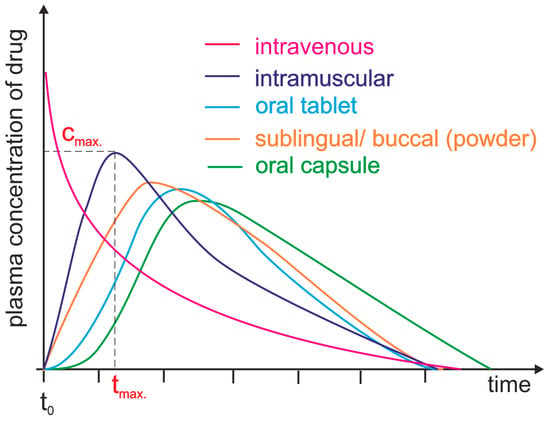
\includegraphics[width=1\linewidth]{images/fig-drug-absorption} \caption{ความเข็มข้นของยาในกระแสเลือดที่เวลาต่างๆ }\label{fig:fig-drug-absorption}
\end{figure}

ในการทำความเข้าใจการเปลี่ยนแปลงของปริมาณข้างต้นเทียบกับเวลา เราสามารถประยุกต์ใช้การสร้างแบบจำลองทางคณิตศาสตร์เพื่อมาใช้อธิบายการเปลี่ยนแปลงของปริมาณต่างๆ ที่เกี่ยวข้อง

\begin{quote}
\textbf{การสร้างแบบจำลองทางคณิตศาสตร์} เป็นกระบวนการอธิบายปัญหาหรือ ปรากฎการต่างๆ ที่เกิดขึ้นในธรรมชาติ โดยปกติแล้วจะอยู่ในรูปของสมการทางคณิตศาสตร์ ซึ่งแบบจำลองทางคณิตศาสตร์นี้จะช่วยให้อธิบายสิ่งต่างๆ ที่เกิดขึ้นในปัญหาหรือปรากฏที่สนใจ
\end{quote}

ตัวอย่างต่อไปนี้จะแสดงถึงแนวคิดในการประยุกต์ของแคลคูลัสที่เกี่ยวข้องกับอัตราการเปลี่ยนแปลงของ

\begin{example}
\protect\hypertarget{exm:exm1}{}\label{exm:exm1}ในการทดลองหนึ่ง นักวิจัยต้องการศึกษาการขยายพันธ์ของแบคทีเรียที่มีการการแบ่งตัวที่เรียกว่า binary fission (การแบ่งตัวแบบทวิภาค) ซึ่งแบคทีเรียจะมีการแบ่งจากหนึ่งเป็นสองเซลเท่าๆ กัน และได้ผลการทำลองดังต่อไปนี้
\end{example}

\begin{figure}
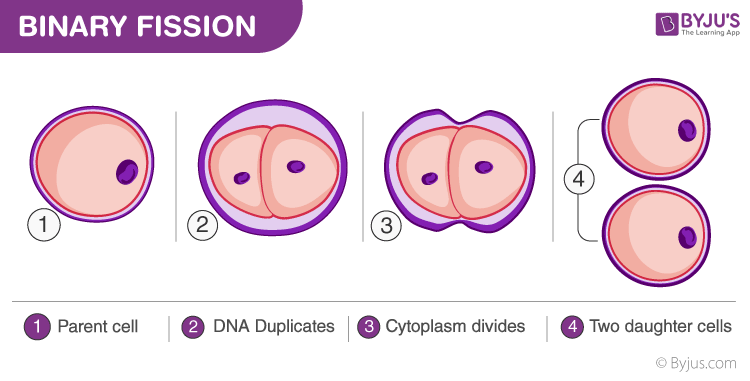
\includegraphics[width=1\linewidth]{images/fig-binary-fission} \caption{กระบวนการแบ่งตัวแบบทวิภาคของแบคทีเรีย}\label{fig:fig-binary-fission}
\end{figure}

(รูปอ้างอิงจาก \href{https://byjus.com/biology/binary-fission/}{BYJU's Learning Website} )

\begin{table}

\caption{\label{tab:bacteria-table}จำนวนของแบคทีเรียที่เวลา t ใดๆ}
\centering
\begin{tabular}[t]{l|r|r|r|r|r|r|r}
\hline
เวลา (10 นาที) & 0 & 1 & 2 & 3 & 4 & 5 & 6\\
\hline
จำนวนแบคทีเรีย & 1 & 2 & 4 & 8 & 16 & 32 & 64\\
\hline
\end{tabular}
\end{table}

ตาราง \ref{tab:bacteria-table} และรูปที่ \ref{fig:population-plot} แสดงการเปลี่ยนแปลงของจำนวนแบคทีเรียที่เวลาใดๆ ในตัวอย่างนี้การเปลี่ยนแปลงของจำนวนของแบคทีเรียที่เวลา \(t\) สามารถเขียนในรูปฟังก์ชัน \(N(t)\) ถ้าให้ \(N_0\) แทนจำนวนของแบคทีเรียตอนเริ่มการทดลอง แล้วแบบจำลองทางคณิตศาสตร์สำหรับการเพิ่มของจำนวนแบคทีเรียจะสามารถเขียนในรูปของสมการ

\begin{equation}
N(t) = N_0 \cdot 2 ^t, \quad t = 0,1,2, \ldots
\label{eq:population-growth}
\end{equation}

ในแบบจำลองทางคณิตศาสตร์นี้การเปลี่ยนแปลงของจำนวนแบคทีเรียที่เวลา \(t\) ใดๆ เพิ่มขึ้นในลักษณะที่เรียกว่า เอกซ์โพเนนเชียล (Exponential Population Growth)

\begin{figure}
\centering
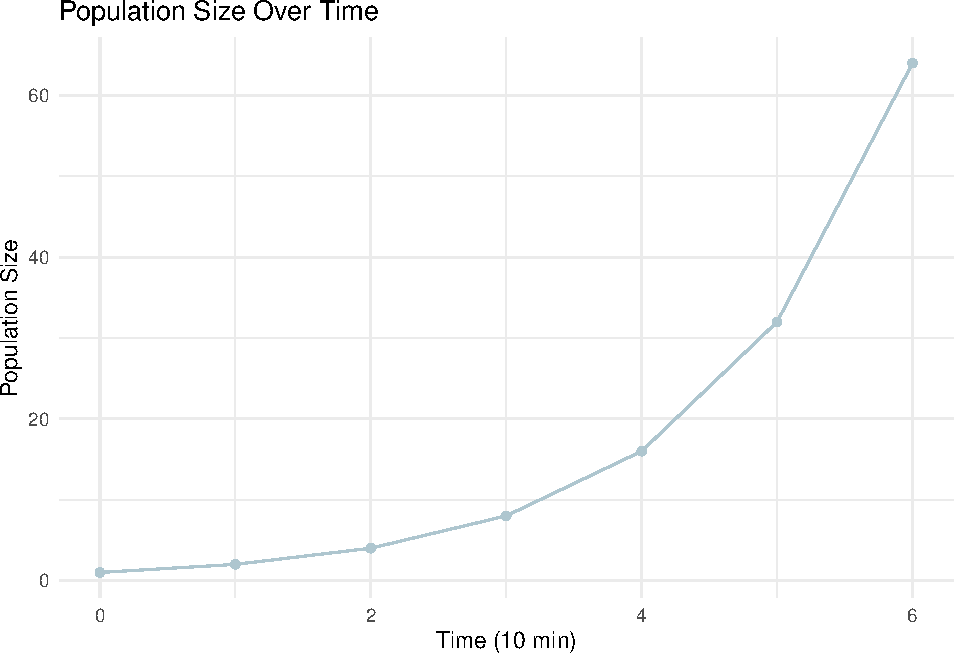
\includegraphics{../SCMA104bookdownproj_files/figure-latex/population-plot-1.pdf}
\caption{\label{fig:population-plot}Population Size Over Time}
\end{figure}

\begin{example}
\protect\hypertarget{exm:exm2}{}\label{exm:exm2}ในการสร้างแบบจำลองทางคณิตศาสตร์ ในตัวอย่างของการขยายพันธ์แบคทีเรีย หรือในปัญหาอื่นๆ แทนที่เราจะพยายามหาความสัมพันธ์ หรือฟังก์ชัน \(N(t)\) ในรูปของเวลา \(t\) โดยตรง ถ้าเราทราบกระบวนการที่เกี่ยวข้องกับการอัตราการเปลี่ยนแปลงของตัวแปร \(N(t)\) นั้น เราสามารถนำมาใช้ในการสร้างแบบจำลองทางคณิตศาสตร์ ได้ดังต่อนี้ กระบวนการที่เกี่ยวข้องกับการเปลี่ยนแปลงของจำนวนแบคทีเรีย (การเพิ่มหรือลดลงของแบคทีเรีย) ที่เกิดขึ้นในระหว่างเวลา \(t\) และเวลา \(t + h\) เกิดจากจำนวนแบคทีเรียที่เพิ่มขึ้น (เกิดขึ้นมาใหม่) ในช่วงเวลาดังกล่าว และลดลงจากจำนวนแบคทีเรียที่ลดลง (ตายไป) ในช่วงเวลาดังกล่าวเช่นกัน ซึ่งเราสามารถเขียนในรูปของสมการได้ดังต่อไปนี้
\end{example}

\begin{align}
N(t + h) &= N(t) \\
&\quad + \text{จำนวนแบคทีเรียที่เกิดขึ้นใหม่ระหว่าง } t \text{ และ } t+h \\
&\quad - \text{จำนวนแบคทีเรียที่ตายไประหว่าง } t \text{ และ } t+h
\label{eq:population-growth-2}
\end{align}

ในที่นี้ ``\textbf{การเกิด}'' เราหมายถึงการเพิ่มจำนวนของแบคทีเรียจากหนึ่งเป็นสอง และเราจะกำหนดให้ \(h\) เป็นช่วงเวลาสั้นๆ (ซึ่งเราสามารถใช้ความรู้แคลคูลัสในการสร้างแบบจำลองทางคณิตศาสตร์ในรูปของสมการเชิงอนุพันธ์ (differential equation)) ในสมการ \eqref{eq:population-growth-2} ถ้าเราสมมติว่า การเพิ่มของแบคทีเรียเป็นสัดส่วนกับจำนวนแบคทีเรียที่มีอยู่ในขณะนั้น หรือเขียนในรูปของสมการได้ดังนี้

\[
\text{จำนวนแบคทีเรียที่เกิดใหม่ระหว่าง } t \text{ และ } t + h \approx b \cdot N \cdot h
\]

\[
\text{จำนวนแบคทีเรียที่ตายไประหว่าง } t \text{ และ } t + h \approx m \cdot N \cdot h
\]

โดยที่ค่าคงตัว \(b\) และ \(m\) ในสมการข้างต้น คือ อัตราการเกิด (birth rate) และอัตราการตาย (mortality rate)

เมื่อแทนจำนวนแบคทีเรียที่เกิดใหม่ และตายไประหว่างช่วงเวลาที่กำหนดลงในสมการ \eqref{eq:population-growth-2} จะได้สมการ

\begin{equation}
N(t + h) - N(t) = b\cdot N(t) \cdot h - m\cdot N(t) \cdot h
\label{eq:population-growth-3}
\end{equation}

เราสามารถจัดรูปสมการ \eqref{eq:population-growth-3} ได้ไหมในรูปของ\textbf{อัตราการเปลี่ยนแปลงเฉลี่ย}ของจำนวนแบคทีเรียในช่วงเวลาดังกล่าว ดังนี้

\begin{align}
\frac{N(t + h) - N(t)}{h} &= b\cdot N(t)  - m\cdot N(t)\\
\label{eq:population-growth-4}
\end{align}

ดังนั้น ถ้าเราให้ \(h\) เข้าใกล้ 0 ผ่านการหาค่าลิมิต เราจะได้อัตราการเปลี่ยนแปลงขณะหนึ่ง (instantaneous rate of change) และเขียนได้ในรูปของสมการเชิงอนุพันธ์ ดังนี้

\begin{align}
\frac{dN}{dt} = \lim_{h \rightarrow 0}\frac{N(t + h) - N(t)}{h} &= b\cdot N(t)  - m\cdot N(t)\\
\label{eq:population-growth-5}
\end{align}

ทั้งนี้ในการแก้สมการเชิงอนุพันธ์ \eqref{eq:population-growth-5} เพื่อให้ได้คำตอบที่แสดงจำนวนแบคทีเรีย \(N(t)\) ในรูปของฟังก์ชันของ \(t\) เราจะต้องกำหนดเงื่อนไขเพิ่มเติมที่เกี่ยวข้องกับจำนวนแบคทีเรีย \(N(t)\) ที่เวลา \(t\) หนึ่ง โดยทั่วไปเราจะกำหนดค่าเริ่มต้นของจำนวนแบคทีเรียที่ \(t = 0\) ดังนั้น ถ้าเรากำหนดเงื่อนไขเริ่มต้น (initial condition)

\begin{equation}
N(0) = N_0
\label{eq:population-growth-6}
\end{equation}

เราสามารถหาคำตอบของสมการเชิงอนุพันธ์ที่มีเงื่อนไขเริ่มต้นโดยวิธีการหาปริพันธ์ (Integration) ได้คำตอบของสมการดังนี้

\begin{equation}
N(t) = N_0 e^{(b-m)t}
\label{eq:population-growth-7}
\end{equation}

\begin{example}
\protect\hypertarget{exm:exm3}{}\label{exm:exm3}

ในการทดลองเลี้ยงยีสต์ในขวดทดลองที่มีอาหารเลี้ยงยีสต์ในปริมาณที่เหมาะสม ผู้ทำการทดลองสนใจที่จะประมาณค่าของยีสต์โดยอาศัยแบบจำลองการเปลี่ยนแปลงของประชากรที่อธิบายด้วยสมการ \eqref{eq:population-growth-7} กำหนดให้

\begin{itemize}
\item
  ภายใต้สภาวะของการทดลองที่เหมาะสม ยีสต์จะแบ่งตัวทุกๆ 90 นาที
\item
  ยีสต์มีครึ่งชีวิตเท่ากับ 1 สัปดาห์
\end{itemize}

จากข้อมูลดังกล่าว จงแสดงวิธีทำเพื่อหาคำตอบจากคำถามต่อไปนี้

\begin{enumerate}
\def\labelenumi{\arabic{enumi}.}
\item
  จงประมาณค่าของอัตราการเกิด \(b\) (1/ชั่วโมง) และอัตราการตาย \(m\) (1/ชั่วโมง)
\item
  เขียนแบบจำลองทางคณิตศาสตร์โดยใช้ค่า \(b\) และ \(m\) ที่ประมาณค่าได้ (สมการ \eqref{eq:population-growth-7})
\item
  ใช้เครื่องมือที่นักศึกษามีอยู่ในการวาดกราฟแสดงความสัมพันธ์ของจำนวนยีสต์ที่เวลาต่างๆ
\item
  เปรียบเทียบผลลัพธ์ที่ได้กับรูปภาพแสดงการเปลี่ยนแปลงของยีสต์จากการทดลองในห้องปฏิการ ตามรูปที่ \ref{fig:fig-yeast-cells} (รูปภาพอ้างอิงจาก \href{https://homework.study.com/explanation/a-graph-of-a-population-of-yeast-cells-in-a-new-laboratory-culture-as-a-function-of-time-is-shown-a-describe-how-the-rate-of-population-increase-varies-b-when-is-this-rate-highest-c-on-what-intervals-is-the-population-function-concave-upward-or-d.html}{https://homework.study.com/})
\end{enumerate}

\end{example}

\begin{figure}
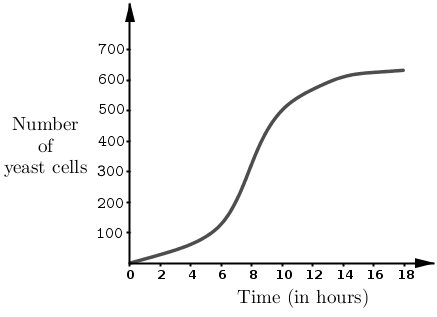
\includegraphics[width=0.5\linewidth]{images/fig-yeast-cells} \caption{กราฟการเจริญเติบโตของเซลล์ยีสต์}\label{fig:fig-yeast-cells}
\end{figure}

\begin{example}
\protect\hypertarget{exm:exm4}{}\label{exm:exm4}

จงใช้อินเทอร์เน็ตเพื่อค้นหาตัวอย่างแบบจำลองทางคณิตศาสตร์ที่อธิบายโดยสมการเชิงอนุพันธ์หรือระบบสมการเชิงอนุพันธ์ ข้อมูลที่ต้องการประกอบด้วย

\begin{enumerate}
\def\labelenumi{\arabic{enumi}.}
\item
  ค้นหาหน้าเว็บที่ให้ข้อมูลเกี่ยวกับแบบจำลองทางคณิตศาสตร์ในปัญหาที่นักศึกษาสนใจ
\item
  จดบันทึก URL ของหน้าเว็บ
\item
  เขียนสรุปสั้นๆ ว่าโมเดลนี้ใช้เพื่ออะไร
\end{enumerate}

\end{example}

โดยสรุป แคลคูลัสและสมการเชิงอนุพันธ์เป็นเครื่องมือสำคัญในการทำความเข้าใจว่าสิ่งต่างๆ เปลี่ยนแปลงไปอย่างไรและ แคลคูลัสช่วยให้เราวิเคราะห์อัตราการเปลี่ยนแปลงและพื้นที่ใต้เส้นโค้ง ในขณะที่สมการเชิงอนุพันธ์ช่วยให้เราสร้างแบบจำลองระบบที่ซับซ้อนในสาขาต่างๆ เช่น ฟิสิกส์ วิศวกรรม เศรษฐศาสตร์ และชีววิทยา แนวคิดทางคณิตศาสตร์เหล่านี้มีความสำคัญต่อการแก้ปัญหาในโลกแห่งความเป็นจริง เมื่อโลกของเราก้าวหน้ามากขึ้น ความสำคัญของแคลคูลัสและสมการเชิงอนุพันธ์ก็จะเพิ่มขึ้นอย่างต่อเนื่อง ซึ่งสนับสนุนความก้าวหน้าทางวิทยาศาสตร์และเทคโนโลยี

\chapter{ลิมิต (Limits)}\label{uxe25uxe21uxe15-limits}

อาจกล่าวได้ว่า วิชาแคลคูลัส
ถือกำเนิดขึ้นมาจากความพยายามในการแก้ปัญหาทางเรขาคณิตบนระนาบ 2 ปัญหาหลักๆ คือ

\begin{itemize}
\item
  การหาเส้นตรงที่สัมผัสเส้นโค้งที่กำหนดให้

  กำหนดฟังก์ชัน (function) \(f\) และกำหนดจุด \(P(x_{0},y_{0})\) บนกราฟ
  \(y = f(x)\) จงหาสมการของเส้นตรงที่สัมผัสกราฟ \(y = f(x)\) ที่จุด \(P\)
\item
  การหาพื้นที่ของบริเวณที่กำหนดให้

  กำหนด function \(f\) และช่วง \([a,b]\) ในโดเมนของ \(f\)
  จงหาพื้นที่ที่ถูกปิดล้อมด้วยแกน \(X\) และกราฟ \(y = f(x)\) สำหรับ \(x \in [a,b]\)
\end{itemize}

แนวความคิดในการแก้ปัญหาทั้งสอง นำไปสู่การศึกษาเรื่อง ลิมิต (Limits)
ซึ่งเป็นพื้นฐานของวิชาแคลคูลัสนั่นเอง

แต่ในปัจจุบันเราพบว่าวิชาแคลคูลัสมีประโยชน์ในการช่วยแก้ปัญหาในสาขาวิชาต่าง ๆ มากมาย เช่น
เราจะพบในการศึกษาวิชานี้ว่า แคลคูลัสมีบทบาทในการแก้ปัญหาต่อไปนี้

\begin{itemize}
\item
  โดยทั่วไป ยาชนิดฉีดจะต้องใช้เวลาระยะหนึ่งหลังจากฉีดเข้าสู่ร่างกาย
  ในการที่จะไหลเวียนในกระแสโลหิต จนกระทั่งมีความเข้มข้นสูงสุด สมมุติว่า
  ยาฉีดชนิดหนึ่งหลังจากฉีดเข้าสู่ร่างกายนาน \(t\) ชั่วโมง จะมีความเข้มข้นเป็น
  \(C(t) = 0.15(e^{-0.18t}-e^{-1.2t})\) มิลลิกรัมต่อมิลลิลิตร จงหาว่า
  นานเท่าใดหลังจากฉีดยา จึงจะมีความเข้มข้นของยา ในกระแสโลหิตสูงที่สุด
\item
  เราอาจประมาณได้อย่างมีเหตุผลว่า artery มีรูปร่างที่เป็นผลมาจากการหมุนรอบแกน
  ของเส้นโค้งในระนาบ โดยในสภาวะนิ่ง รัศมีของ artery มีค่าคงที่เท่ากับ 1 หน่วย
  (รูปทรงกระบอก) แต่ในขณะที่หัวใจสูบฉีดโลหิตผ่าน artery artery จะพองตัวออก
  ทำให้รัศมีเปลี่ยนไปตามสมการ \(R(x) = 1+0.4x-0.04x^{2}\) หน่วย เมื่อ
  \(0 \leq x\leq 10\) เป็นตำแหน่งบนแนวยาวของ artery จงหาว่า ปริมาณโลหิตที่อยู่ใน
  artery ขณะที่หัวใจสูบฉีดโลหิตผ่านเข้ามาเป็นกี่เท่าของความจุโลหิตในสภาวะนิ่ง
\item
  ความก้าวหน้าในทางการแพทย์ และเทคโนโลยีปัจจุบัน
  ทำให้มีการประดิษฐ์อุปกรณ์ช่วยในการรักษาโรคเบาหวานชิ้นหนึ่งขึ้น
  อุปกรณ์นี้มีลักษณะเป็นแคปซูล ซึ่งเมื่อฝังอุปกรณ์นี้ภายในร่างกายแล้ว
  มันจะหลั่งสารอินซูลินที่บรรจุอยู่ภายใน ออกสู่กระแสโลหิต โดยมีอัตราการหลั่งเป็น
  \(f\left( t\right) =0.5te^{-0.09t}\) ลูกบาศก์เซนติเมตรต่อวัน เมื่อ t คือ
  เวลาเป็นวัน นับจากอุปกรณ์เริ่มทำงาน จงหาว่า
  แพทย์จะต้องสั่งให้บรรจุอินซูลินในแคปซูลเป็นปริมาณเท่าใด
  เพื่อให้อุปกรณ์นี้สามารถให้อินซูลินแก่ผู้ป่วยได้นาน 3 เดือน
\item
  การหาเส้นตรงที่สัมผัสเส้นโค้ง \(y = f(x)\) ณ จุด \(P_{0}(x_{0},y_{0})\)
\end{itemize}

\begin{figure}
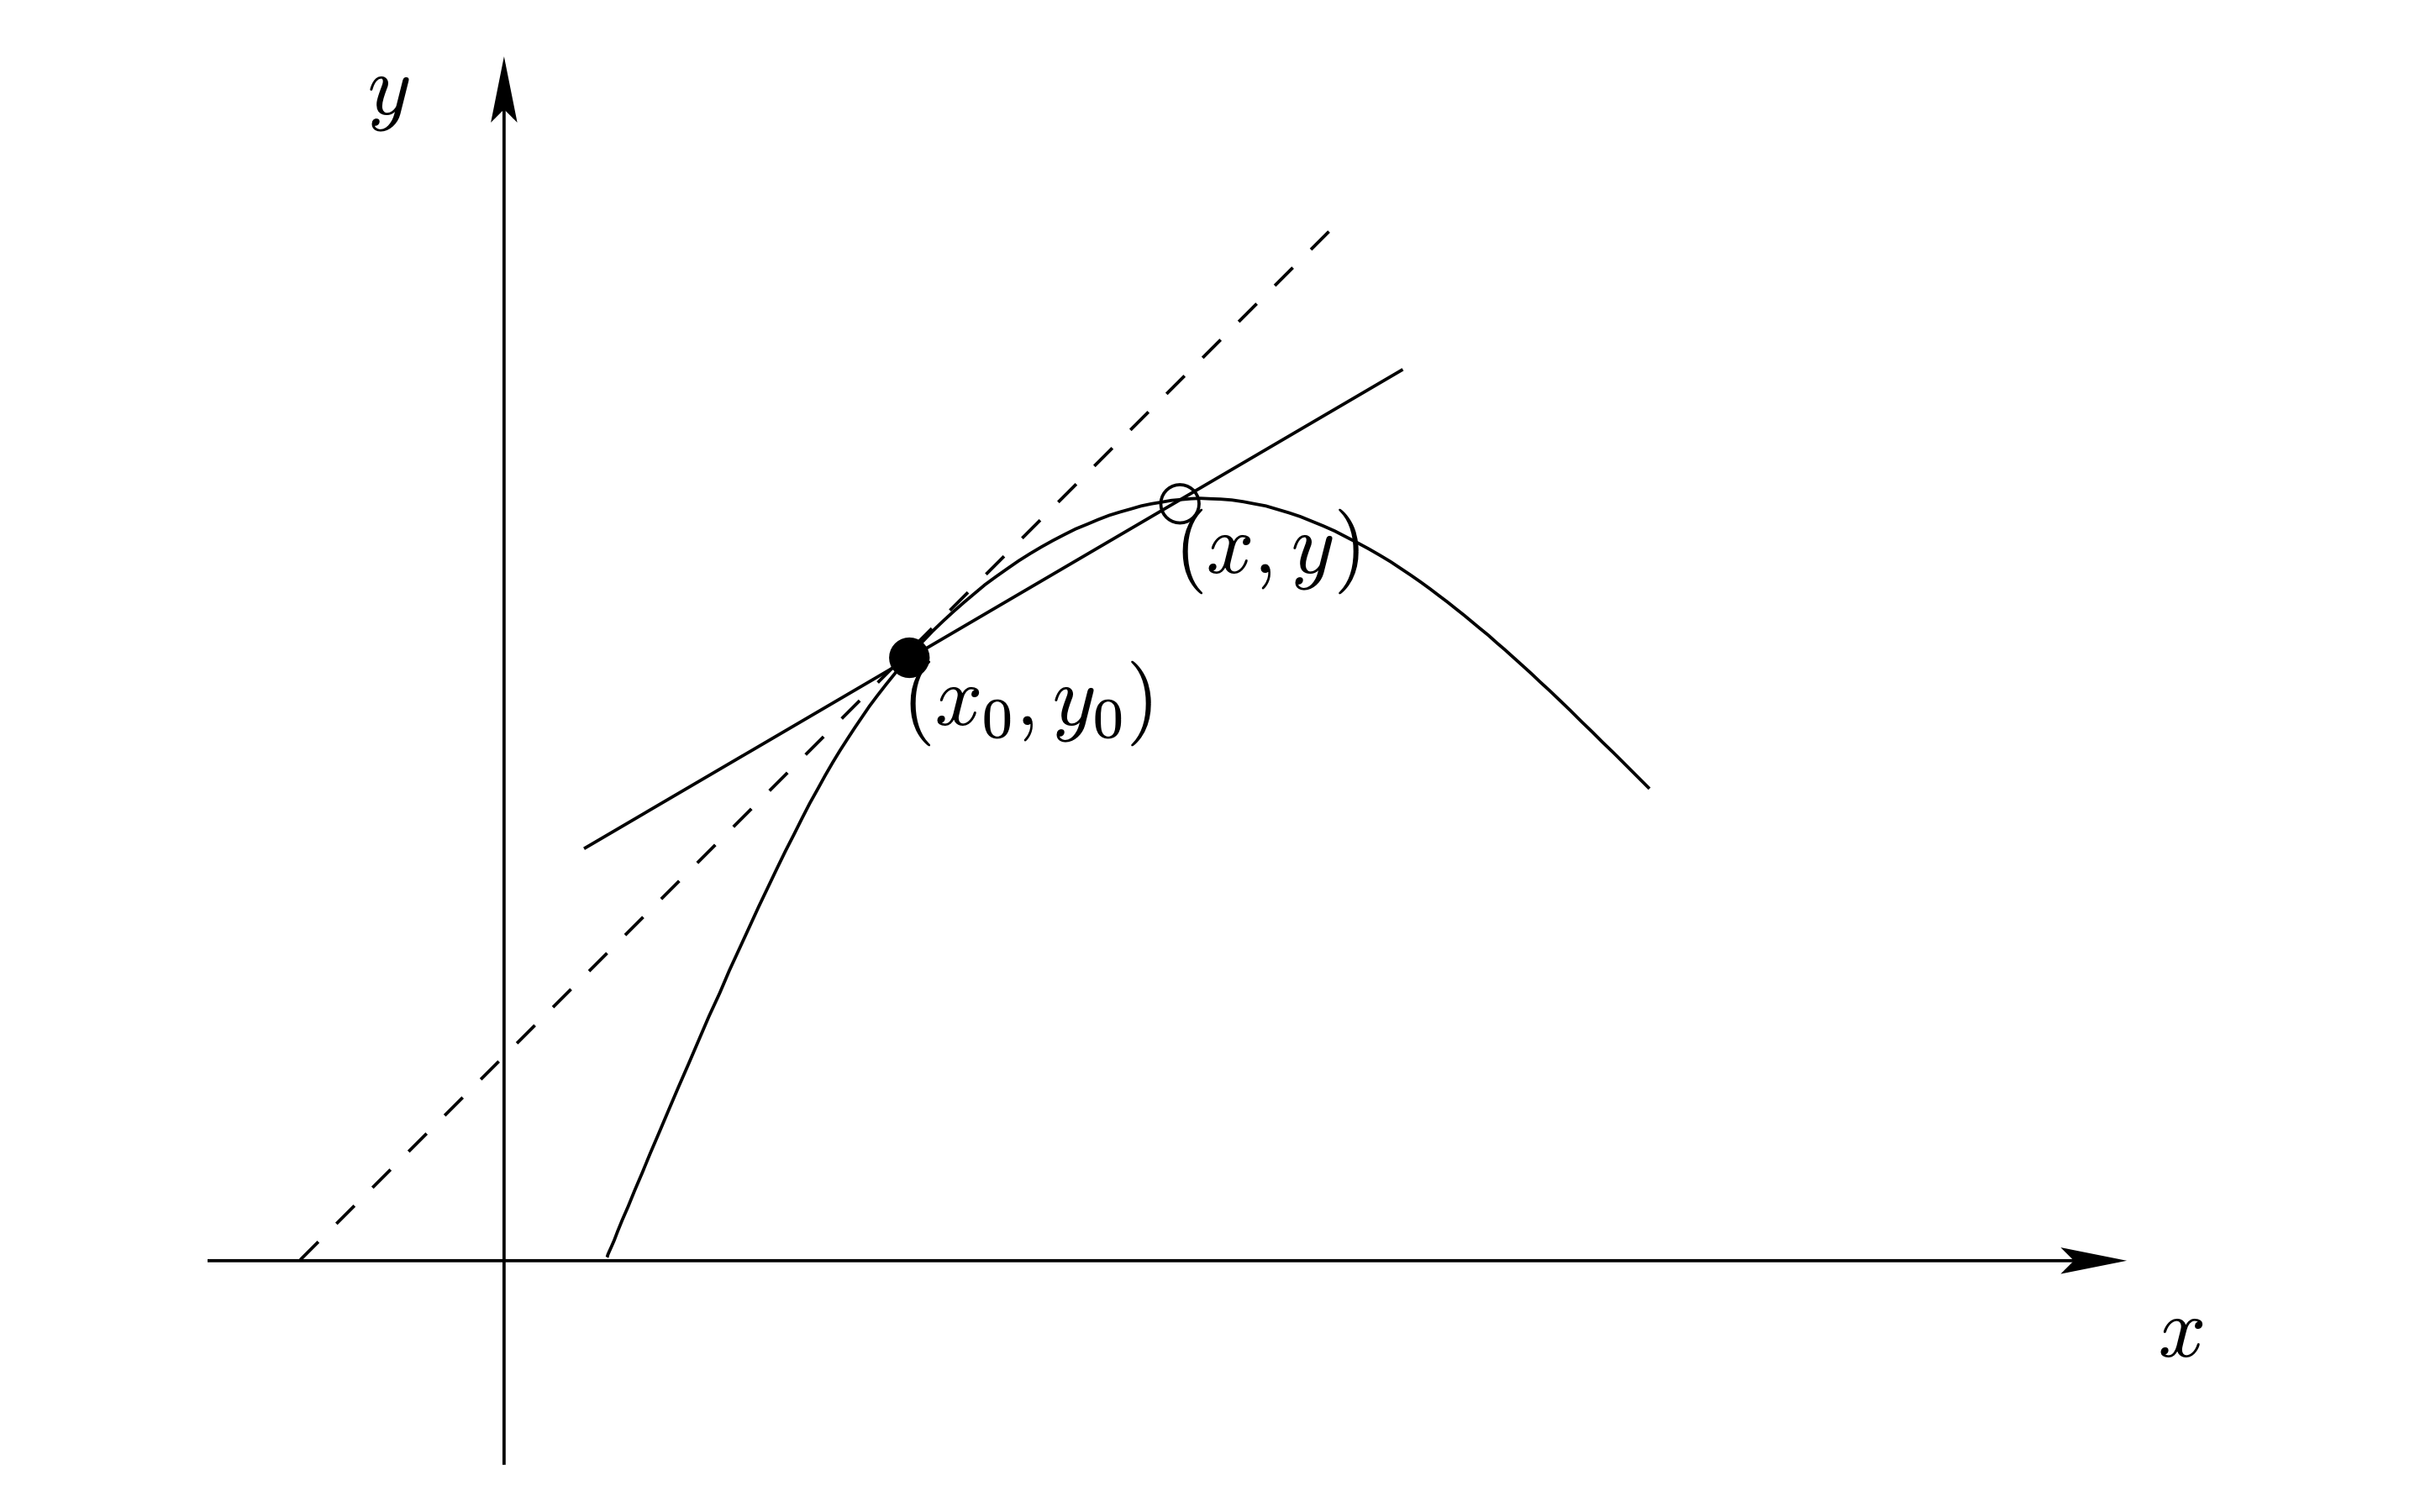
\includegraphics[width=0.5\linewidth]{images/fig-tangent-line} \caption{การหาเส้นตรงที่สัมผัสเส้นโค้ง}\label{fig:fig-tangent-line}
\end{figure}

ขั้นตอนสรุปการหาเส้นตรงที่สัมผัสเส้นโค้ง

\begin{enumerate}
\def\labelenumi{\arabic{enumi}.}
\item
  เลือกจุดอื่นบนกราฟ เรียกจุดนี้ว่า \(P(x,y)\)
\item
  ลากเส้นผ่าน \(PP_{0}\)
\item
  ทำซ้ำโดยเลือกจุด P ให้ใกล้ \(P_{0}\) มากขึ้น
\item
  เส้น \(PP_{0}\) ที่ได้จะ ``เข้าใกล้'' เส้นสัมผัสมากขึ้นทุกที
\end{enumerate}

\begin{itemize}
\tightlist
\item
  การหาพื้นที่ ``ใต้กราฟ'' ระหว่าง x = a กับ x = b
\end{itemize}

\begin{figure}
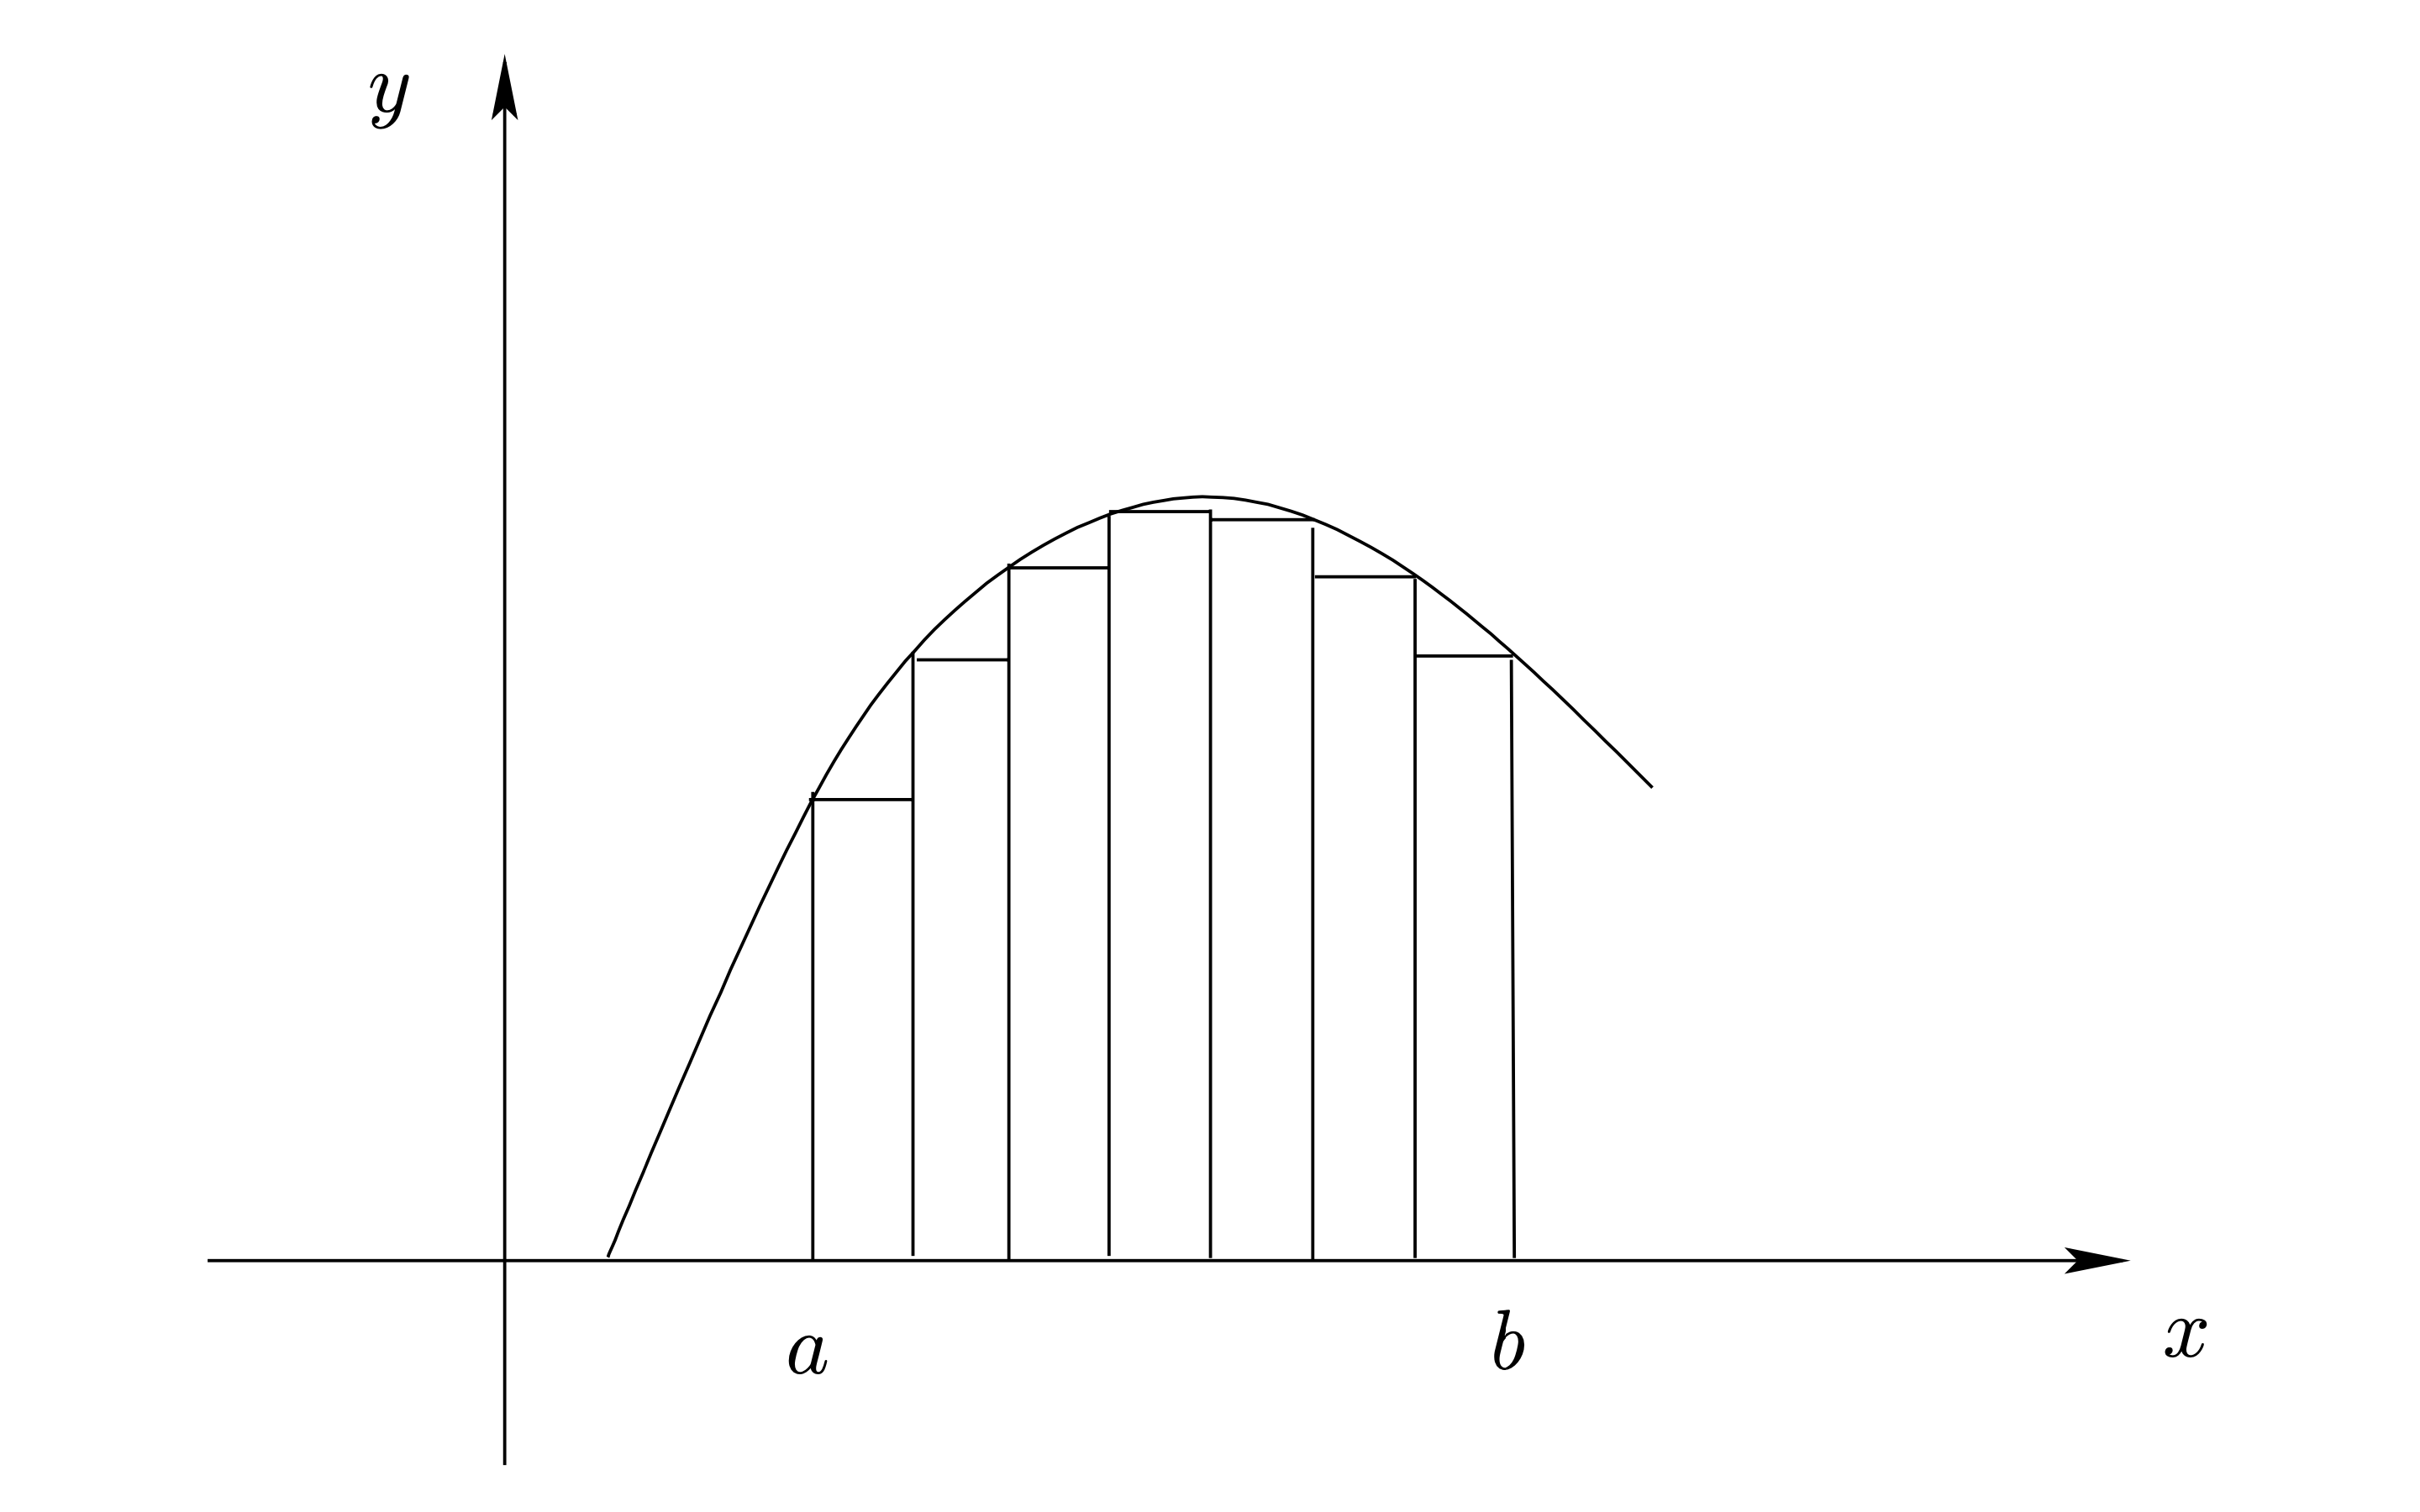
\includegraphics[width=0.5\linewidth]{images/fig-area-under-curve} \caption{การหาพื้นที่ใต้กราฟ}\label{fig:fig-area-under-curve}
\end{figure}

ขั้นตอนเบื้องต้นสำหรับการหาพื้นที่ใต้กราฟ

\begin{enumerate}
\def\labelenumi{\arabic{enumi}.}
\tightlist
\item
  แบ่ง \([a,b]\) เป็นช่วงเล็กๆ
\item
  หาพื้นที่รวมของสี่เหลี่ยมผืนผ้าทั้งหมด
\item
  ทำซ้ำๆ โดยแบ่งช่วงให้เล็กมากขึ้น
\item
  พื้นที่ที่ได้จะ ``เข้าใกล้'' พื้นที่ที่ต้องการมากขึ้นทุกที
\end{enumerate}

\begin{example}
\protect\hypertarget{exm:ex-limit-1}{}\label{exm:ex-limit-1}จงหาสมการของเส้นสัมผัสกราฟ \(y=-x^{2}+6x-2\) ณ จุด \(P_{0}(2,6)\)
\end{example}

\textbf{วิธีทำ}  เลือกจุด \(P(x,y)\) โดยที่ \(x \neq 2\) และลากเส้น \(PP_{0}\) จะได้ว่า
ความชันของ \(PP_{0}\) เท่ากับ \[\begin{aligned}
    \frac{y-6}{x-2} &= \frac{-x^{2}+6x-8}{x-2} \\
                    &=-\frac{\left( x-2\right) \left( x-4\right) }{x-2} \\
                    &=4-x
\end{aligned}\] ถ้า \(P\) อยู่ใกล้ \(P_{0}\) มากขึ้น ค่า x ย่อมเกือบเป็น 2 ดังนั้น
ความชันของ \(PP_{0}\) จึงเข้าใกล้ 4-2 = 2 มากขึ้นเรื่อย ๆ เส้นสัมผัสจึงควรมีความชันเป็น 2
และสมการเส้นสัมผัส คือ \(y-6=2\left( x-2\right)\)

\begin{figure}
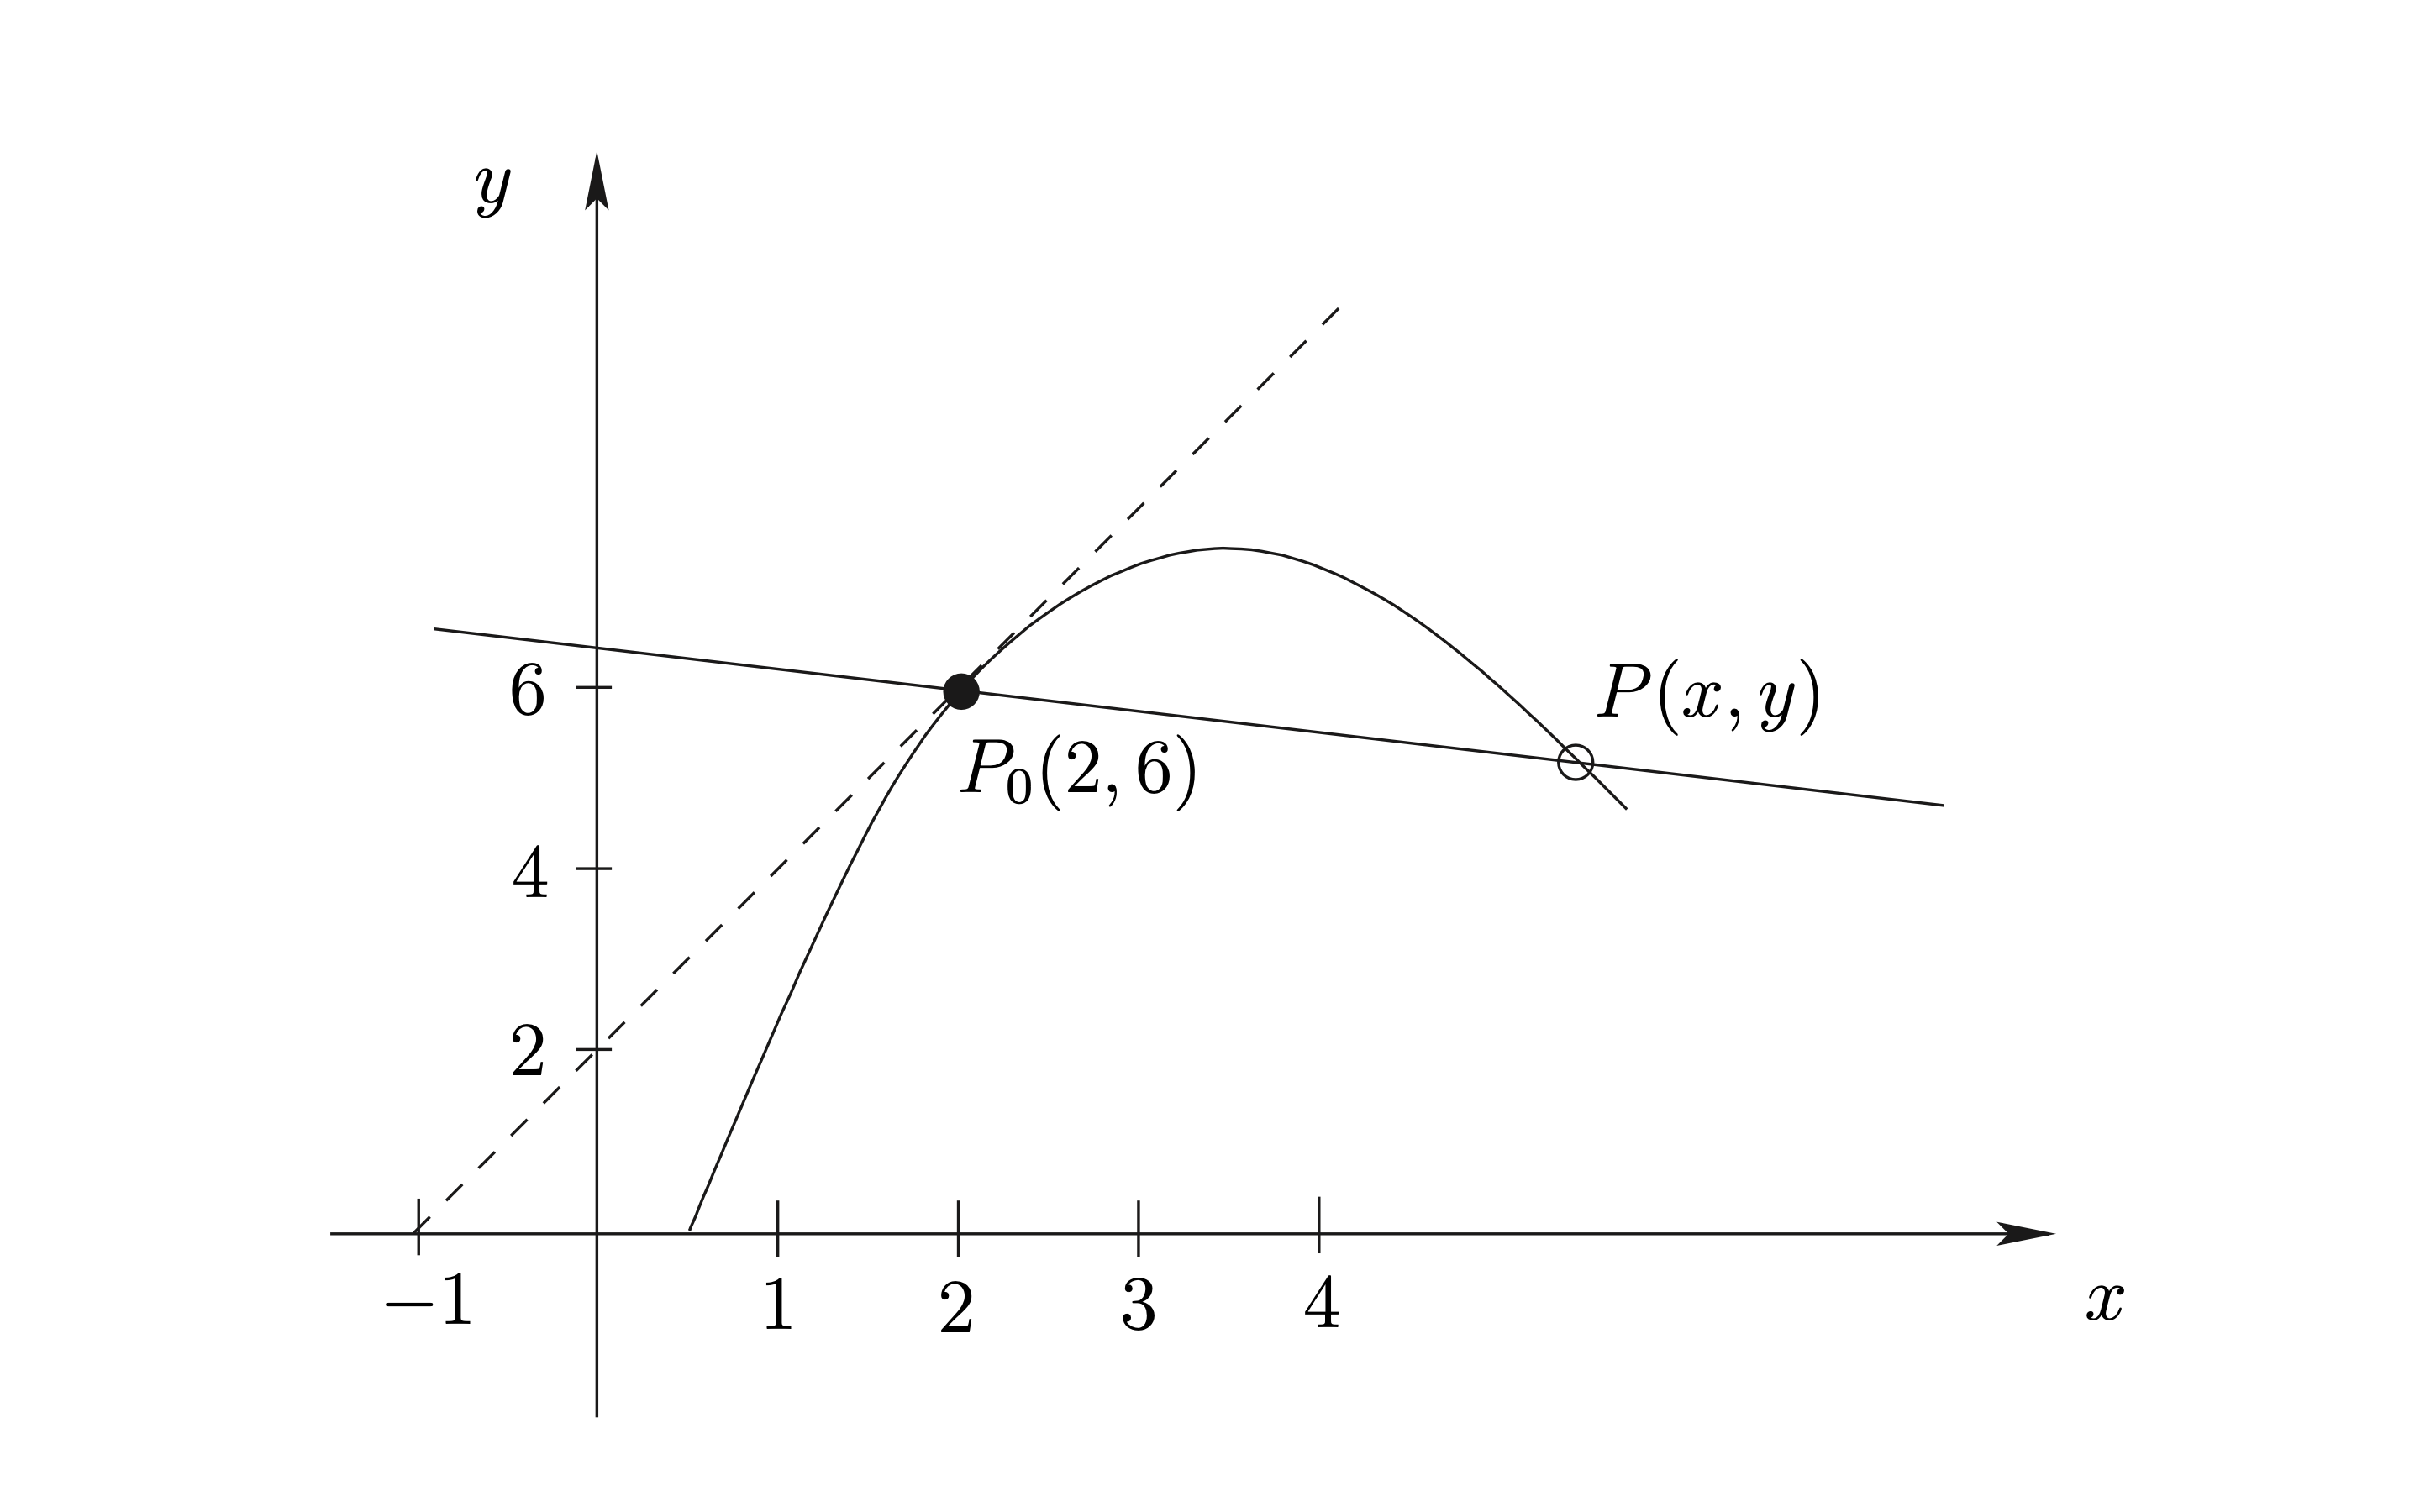
\includegraphics[width=0.5\linewidth]{images/fig-tangent-line-2} \caption{การหาเส้นตรงที่สัมผัสเส้นโค้ง \(y=-x^{2}+6x-2\)}\label{fig:fig-tangent-line-2}
\end{figure}

จะเห็นว่า ในตัวอย่าง \ref{exm:ex-limit-1} นี้ เราสนใจพฤติกรรมของ function

\(\frac{-x^{2}+6x-8}{x-2}\) เมื่อ \(x \neq 2\) แต่มีค่าใกล้ 2 มาก ๆ นี่คือ ที่มาของเรื่อง

\begin{definition}
\protect\hypertarget{def:def-limit}{}\label{def:def-limit}ให้ \(f : D_{f}\rightarrow R\) โดยที่ \(D_{f}\subseteq R\) และให้ \(a \in R\)
โดยที่มีช่วง \((a,b)\) บางช่วงที่ \(\left( a,b\right) \subseteq D_{f}\left( b>a\right)\)

เรากล่าวว่า "ลิมิต (limit) ของ \(f(x)\) เมื่อ x เข้าใกล้ a ทางขวา หาค่าได้และมีค่าเท่ากับจำนวนจริง L" ถ้า "ไม่ว่าเราจะกำหนดบริเวณรอบ ๆ \(L\)
ไว้แคบเพียงใด เมื่อเราพิจารณาค่าของ \(f(x)\) สำหรับค่า \(x\) ที่มากกว่า a โดยที่ให้ค่า ของ \(x\) ลดลงเรื่อย ๆ จนถีงจุดหนึ่ง ค่าของ \(f(x)\) จะอยู่ในบริเวณรอบ ๆ \(L\) ที่เรากำหนดไว้นั้น และยังคงเป็นเช่นนี้สำหรับ \(x\) อื่น ๆ ที่น้อยกว่านั้น (แต่มากกว่า \(a\) ) ทั้งหมดด้วย"

ในทำนองเดียวกัน ถ้าเราพิจารณาพฤติกรรมของ function สำหรับ \(x\) ที่น้อยกว่า \(a\) จะได้ limit ทางซ้าย ดังนี้ ให้ \(f : D_{f}\rightarrow R\) โดยที่ \(D_{f}\subseteq R\) และให้ \(a \in R\) โดยที่มีช่วง \((b,a)\) บางช่วงที่ \(\left( b,a\right) \subseteq D_{f}\left( b<a\right)\)

เรากล่าวว่า "limit ของ \(f(x)\) เมื่อ \(x\) เข้าใกล้ a ทางซ้าย หาค่าได้ และมีค่าเท่ากับจำนวนจริง \(L\)" ถ้า "ไม่ว่าเราจะกำหนดบริเวณรอบ ๆ \(L\) ไว้แคบเพียงใด

เมื่อเราพิจารณาค่าของ \(f(x)\) สำหรับค่า \(x\) ที่น้อยกว่า \(a\) โดยที่ให้ค่า ของ \(x\) เพิ่มขึ้นเรื่อย ๆ จนถีงจุดหนึ่ง ค่าของ \(f(x)\) จะอยู่ในบริเวณรอบ ๆ \(L\) ที่เรากำหนดไว้นั้น และยังคงเป็นเช่นนี้สำหรับ \(x\) อื่น ๆ ที่มากกว่านั้น (แต่น้อยกว่า \(a\) ) ทั้งหมดด้วย"
\end{definition}

เราใช้สัญลักษณ์ \(\underset{x\rightarrow a^{+}}{\lim}f(x)\) แทนข้อความ "limit
ของ \(f(x)\) เมื่อ \(x\) เข้าใกล้ a ทางขวา" และใช้สัญลักษณ์ \(\underset{x\rightarrow a^{-}}{\lim}f(x)\) แทนข้อความ "limit ของ \(f(x)\)
เมื่อ \(x\) เข้าใกล้ a ทางซ้าย

\begin{definition}
\protect\hypertarget{def:def-limit-2}{}\label{def:def-limit-2}ในกรณีที่ทั้ง \(\underset{x\rightarrow a^{+}}{\lim}f(x)\) และ \(\underset{x\rightarrow a^{-}}{\lim}f(x)\) หาค่าได้ และมีค่าเท่ากัน

เรากล่าวว่า \(\underset{x\rightarrow a}{\lim}f(x)\) หาค่าได้ และมีค่าเท่ากับค่านั้น
\end{definition}

\begin{example}
\protect\hypertarget{exm:ex-limit-2}{}\label{exm:ex-limit-2}function \(f\) ที่ \(\underset{x\rightarrow a^{+}}{\lim}f(x)\) หาค่าไม่ได้ ดังนั้น

\(\underset{x\rightarrow a}{\lim}f(x)\) จึงหาค่าไม่ได้ด้วย
\end{example}

\textbf{วิธีทำ}  จากรูปต่อไปนี้

\begin{figure}

{\centering 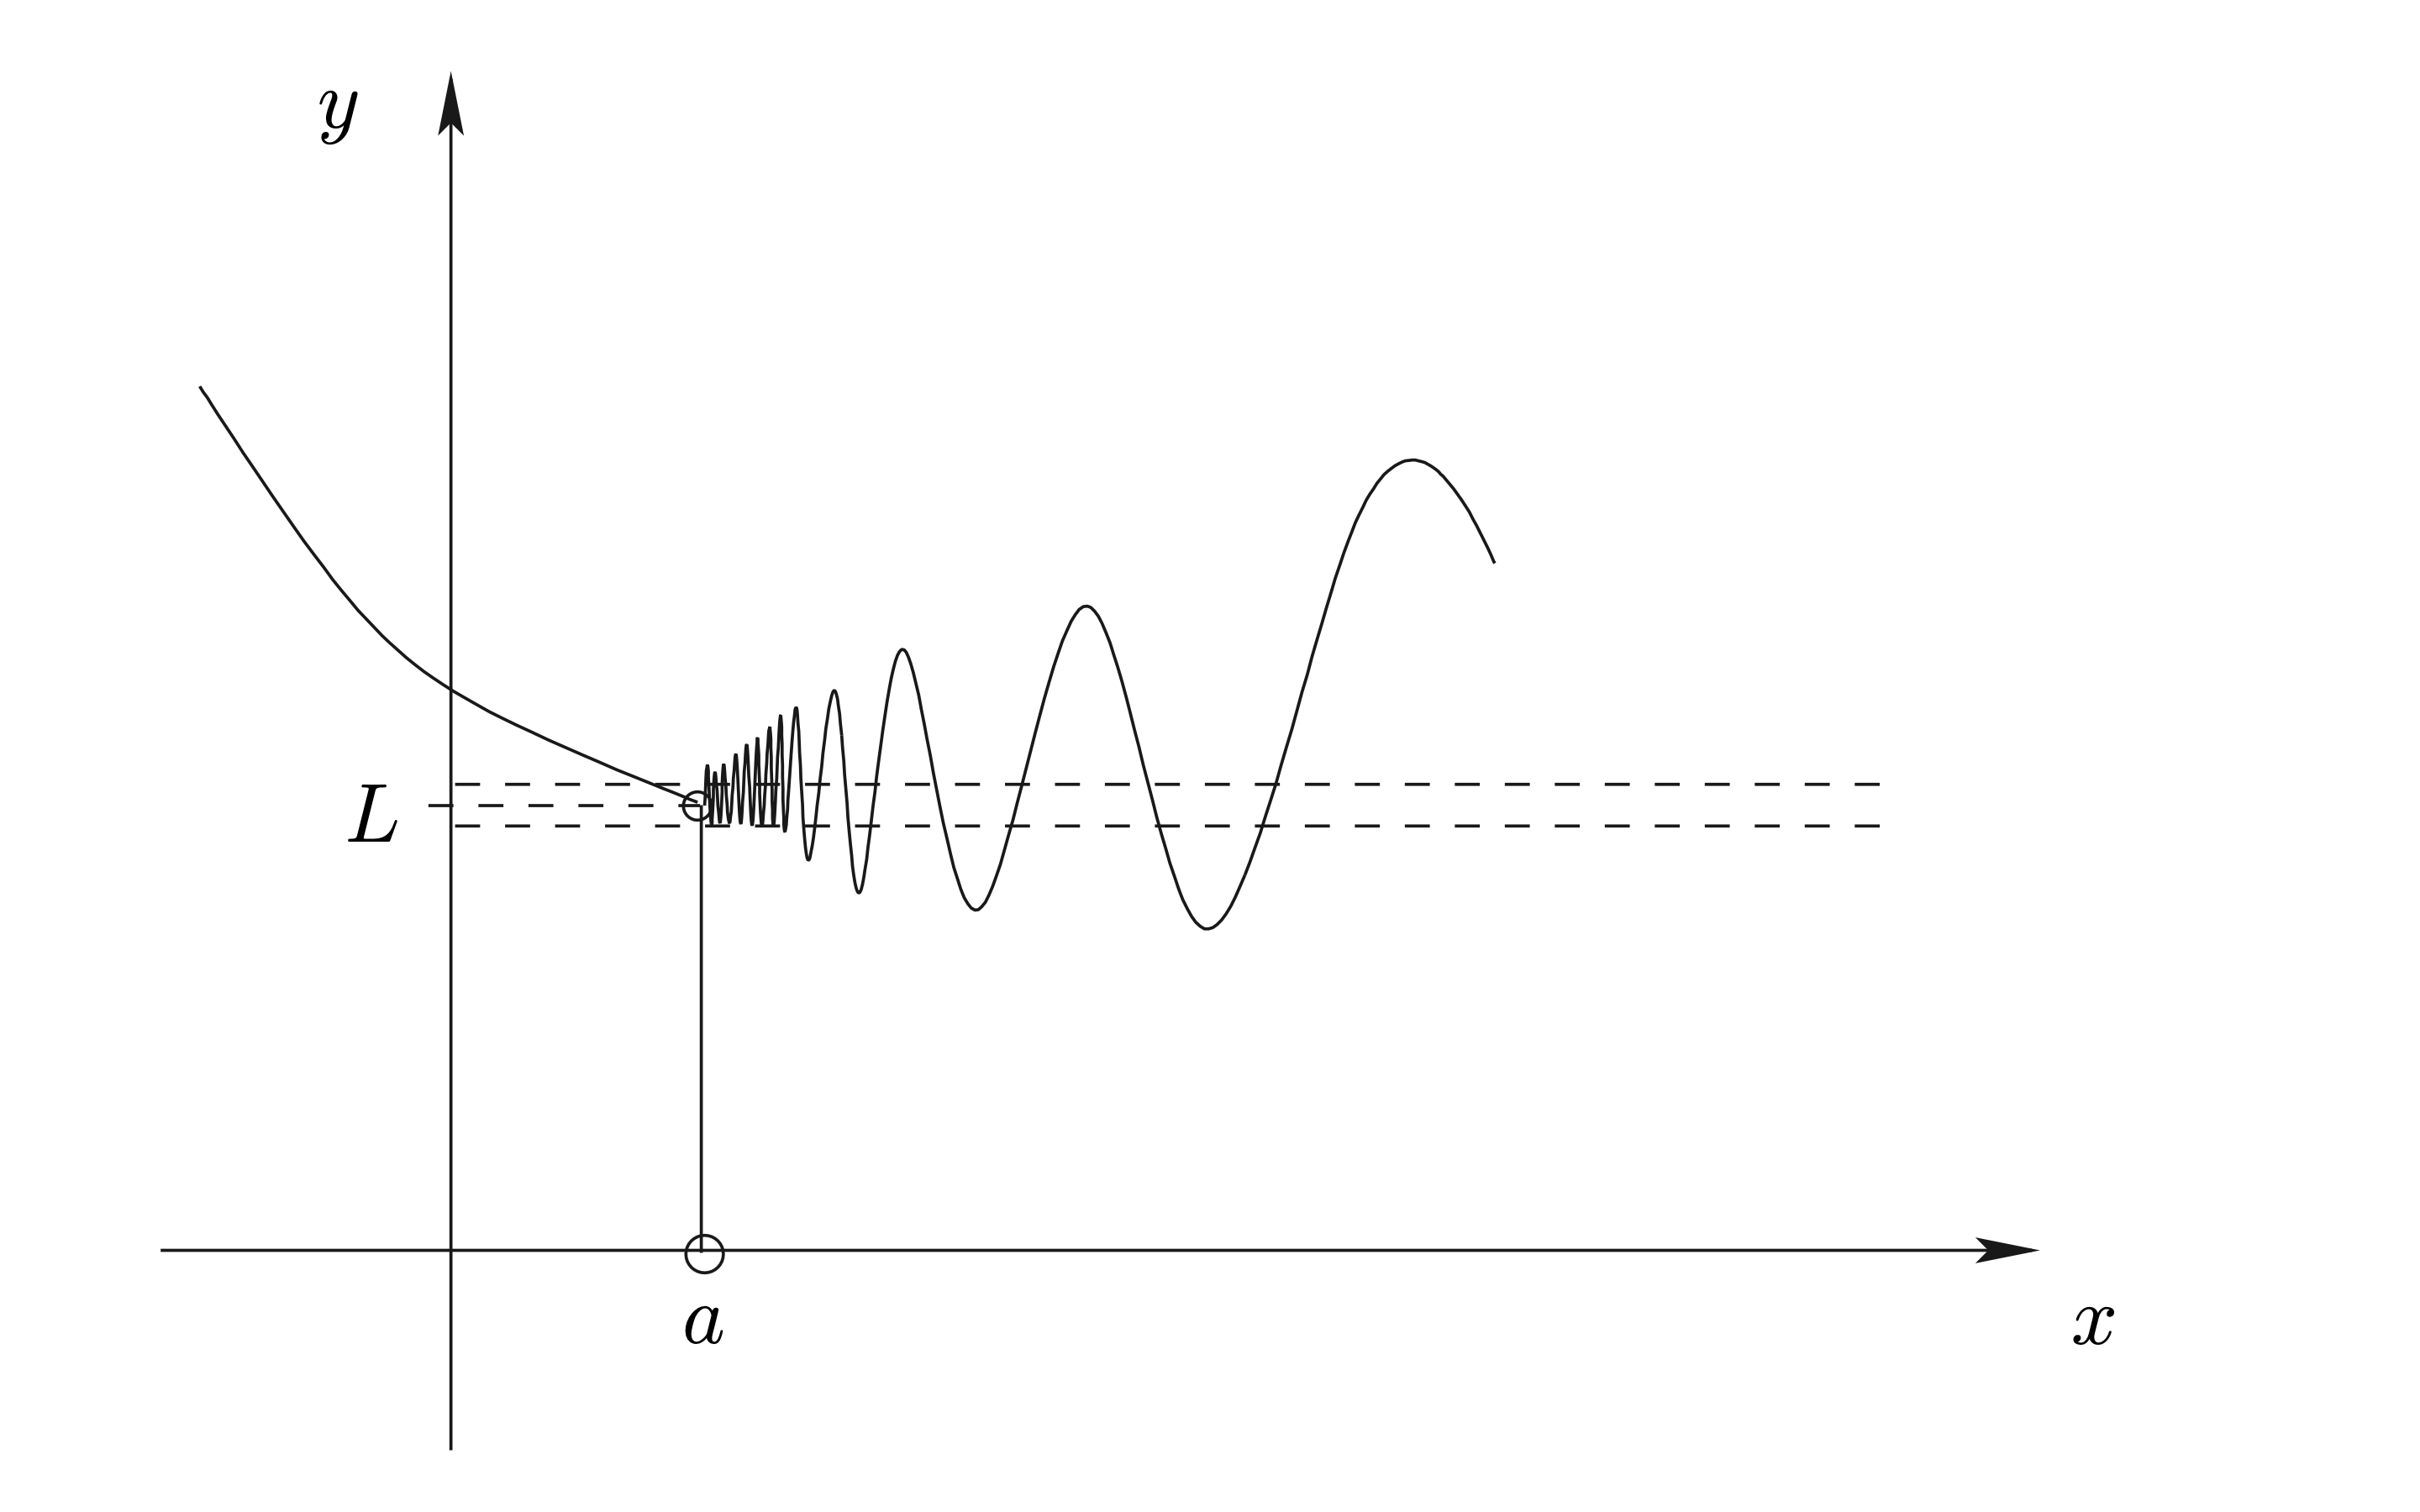
\includegraphics[width=0.5\linewidth]{images/fig-limit-1} 

}

\caption{กราฟของฟังก์ชันที่หาลิมิตไม่ได้}\label{fig:fig-limit-1}
\end{figure}

ในกรณีนี้ จะเห็นว่า ไม่ว่าจะเลือก \(L\) เป็นค่าใด ก็ไม่สามารถสรุปได้ว่า
\(\underset{x\rightarrow 0^{+}}{\lim}f(x)=L\)
เพราะไม่ใช่ทุกครั้งที่เรากำหนดบริเวณรอบ ๆ \(L\) แล้ว function
จะสอดคล้องตามนิยามเสมอไป จึงสรุปว่า \(\underset{x\rightarrow a}{\lim}f(x)=L\)
หาค่าไม่ได้ด้วย

\begin{theorem}
\protect\hypertarget{thm:thm-limit-1}{}\label{thm:thm-limit-1}\leavevmode

\begin{enumerate}
\def\labelenumi{\arabic{enumi}.}
\item
  \(\underset{x\rightarrow c}{\lim}c=c\) ถ้า c เป็นจำนวนจริง
\item
  \(\underset{x\rightarrow a}{\lim}x=a\)
\end{enumerate}

\end{theorem}

\begin{theorem}
\protect\hypertarget{thm:thm-limit-2}{}\label{thm:thm-limit-2}

ถ้า \(\underset{x\rightarrow a}{\lim}f(x)\) และ
\(\underset{x\rightarrow a}{\lim}g(x)\) หาค่าได้แล้ว จะได้

\begin{enumerate}
\def\labelenumi{\arabic{enumi}.}
\item
  \(\underset{x\rightarrow a}{\lim}(f+g)(x)=\underset{x\rightarrow a}{\lim}f(x)+\underset{x\rightarrow a}{\lim}g(x)\)
\item
  \(\underset{x\rightarrow a}{\lim}(f-g)(x)=\underset{x\rightarrow a}{\lim}f(x)-\underset{x\rightarrow a}{\lim}g(x)\)
\item
  \(\underset{x\rightarrow a}{\lim}(f\cdot g)(x)=\left( \underset{x\rightarrow a}{\lim}f(x)\right) \cdot \left( \underset{x\rightarrow a}{\lim}g(x)\right)\)
\item
  \(\underset{x\rightarrow a}{\lim}\left( \frac{f}{g}\right) (x)=\frac{\underset{x\rightarrow a}{\lim}f(x)}{\underset{x\rightarrow a}{\lim}g(x)}\)
  ถ้า \(\underset{x\rightarrow a}{\lim}g(x)\neq 0\)
\end{enumerate}

\end{theorem}

\textbf{หมายเหตุ} ทฤษฎีบททั้งสองนี้ยังคงเป็นจริงสำหรับ limit ทางซ้าย และ limit ทางขวาด้วย

\begin{theorem}
\protect\hypertarget{thm:thm-limit-3}{}\label{thm:thm-limit-3}ถ้า \(\underset{x\rightarrow a}{\lim}f(x)\) หาค่าได้ และ
\(\root{n}\of{f\left( x\right) }\) หาค่าได้ สำหรับทุก ๆ \(x\) ในช่วงเปิดบางช่วงที่มี
\(a\) อยู่ด้วย แล้ว
\(\underset{x\rightarrow a}{\lim}\root{n}\of{f\left( x\right) }=\root{n}\of{\underset{x\rightarrow a}{\lim}f(x)}\)
\end{theorem}

\textbf{หมายเหตุ} ทฤษฎีบทนี้เป็นจริงสำหรับ limit ทางซ้าย และ limit ทางขวาด้วย
โดยเปลี่ยนเงื่อนไข ``ทุก ๆ \(x\)'' เป็น ``ทุก ๆ \(x < a\)'' และ ``ทุก ๆ \(x > a\)'' ตามลำดับ

\begin{theorem}
\protect\hypertarget{thm:thm-limit-4}{}\label{thm:thm-limit-4}ถ้า \(f\) และ \(g\) เป็น function ซึ่ง \(f\left( x\right) =g\left( x\right)\)
สำหรับทุก ๆ \(x\) ยกเว้นบาง \(x\) ซึ่งมีอยู่เพียงจำนวนจำกัด แล้ว
\(\underset{x\rightarrow a}{\lim}f(x)=\underset{x\rightarrow a}{\lim}g(x)\)
ถ้า limit อันใดอันหนึ่งหาค่าได้
\end{theorem}

\textbf{หมายเหตุ} ทฤษฎีบทนี้ยังคงเป็นจริงสำหรับ limit ทางซ้าย และ limit ทางขวาด้วย

\begin{example}
\protect\hypertarget{exm:ex-limit-3}{}\label{exm:ex-limit-3}จงหาค่าของ \(\underset{x\rightarrow 2}{\lim}\frac{-x^{2}+6x-8}{x-2}\)
\end{example}

\textbf{วิธีทำ} 

\begin{equation}
  \begin{aligned}
    \lim_{x\rightarrow 2}\frac{-x^{2}+6x-8}{x-2}
    &= \lim_{x\rightarrow 2} -\frac{\left( x-2\right) \left( x-4\right) }{x-2}\\
    &= \lim_{x\rightarrow 2} -\left( x-4\right) \\ %ต่างกับ function เดิม ที่ค่าเดียของ x คือ x = 2
    &= \lim_{x\rightarrow 2}\left( 4-x\right) \\
    &= \lim_{x\rightarrow 2}4-\lim_{x\rightarrow 2}x\\
    &= 4-2 \\
    &= 2
  \end{aligned}
\end{equation}

\begin{example}
\protect\hypertarget{exm:ex-limit-4}{}\label{exm:ex-limit-4}จงหาค่าของ \(\underset{x\rightarrow 3}{\lim}\frac{\sqrt{x}-\sqrt{3}}{x-3}\)
\textbf{วิธีทำ} 

\begin{equation}
  \begin{aligned}
    \lim_{x\rightarrow 3}\frac{\sqrt{x}-\sqrt{3}}{x-3}
    &= \lim_{x\rightarrow 3}\frac{\sqrt{x}-\sqrt{3}}{x-3}\cdot \frac{\sqrt{x}+\sqrt{3}}{\sqrt{x}+\sqrt{3}} \\
    &= \lim_{x\rightarrow 3}\frac{x-3}{\left( x-3\right) \left( \sqrt{x}+\sqrt{3}\right) } \\
    &= \lim_{x\rightarrow 3}\frac{1}{\sqrt{x}+\sqrt{3}}\\
    &= \frac{\lim_{x\rightarrow 3}1}{\lim_{x\rightarrow 3} \sqrt{x} + \lim_{x\rightarrow 3} \sqrt{3}} \\
    &= \frac{\lim_{x\rightarrow 3}1}{\sqrt{\lim_{x\rightarrow 3}x}+\lim_{x\rightarrow 3}\sqrt{3}} \\
    &= \frac{1}{\sqrt{3}+\sqrt{3}} \\
    &= \frac{1}{2\sqrt{3}} \\
  \end{aligned}
\end{equation}
\end{example}

\begin{example}
\protect\hypertarget{exm:ex-limit-5}{}\label{exm:ex-limit-5}

จงหา limits ต่อไปนี้

\begin{enumerate}
\def\labelenumi{\arabic{enumi}.}
\item
  \(\underset{x\rightarrow 0^{+}}{\lim}\frac{\sqrt{x}-\sqrt{3}}{x-3}\)
\item
  \(\underset{x\rightarrow 0^{-}}{\lim}\frac{\sqrt{x}-\sqrt{3}}{x-3}\)
\item
  \(\underset{x\rightarrow 0}{\lim}\frac{\sqrt{x}-\sqrt{3}}{x-3}\)
\end{enumerate}

\end{example}

\textbf{วิธีทำ} 

\begin{enumerate}
\def\labelenumi{\arabic{enumi}.}
\item
  \(\underset{x\rightarrow 0^{+}}{\lim}\frac{\sqrt{x}-\sqrt{3}}{x-3}\)\(=\frac{0-\sqrt{3}}{x-3}=\frac{\sqrt{3}}{3}\)
\item
  เนื่องจาก function \(\frac{\sqrt{x}-\sqrt{3}}{x-3}\) ไม่ใช่ function
  ที่หาค่าได้บนช่วงเปิด \(\left( b,0\right)\) ใด ๆ เลย ดังนั้น
  \(\underset{x\rightarrow 0^{-}}{\lim}\frac{\sqrt{x}-\sqrt{3}}{x-3}\)
  จึงหาค่าไม่ได้
\item
  เนื่องจาก
  \(\underset{x\rightarrow 0^{-}}{\lim}\frac{\sqrt{x}-\sqrt{3}}{x-3}\)
  หาค่าไม่ได้ ดังนั้น
  \(\underset{x\rightarrow 0}{\lim}\frac{\sqrt{x}-\sqrt{3}}{x-3}\)
  จึงหาค่าไม่ได้
\end{enumerate}

\textbf{ข้อสังเกต} ในกรณีที่ function ที่มีค่ามากขึ้นโดยไม่มีขอบเขต เมื่อตัวแปรต้นเข้าใกล้ \(a\)
(ทางซ้ายหรือขวา หรือทั้งสองทาง) บางตำรากล่าวว่า limit ของ function มีค่าเป็น
\(+\infty\) และถ้า function มีค่าลดลงโดยไม่มีขอบเขต จะกล่าวว่า limit ของ function
มีค่าเป็น \(-\infty\) ในวิชานี้เราจะถือตามนิยามที่ให้ไว้ ดังนั้นในกรณีข้างต้น จะกล่าวว่า limit
ดังกล่าวหาค่าไม่ได้ (เว้นแต่จะระบุให้พิจารณาค่า \(\pm \infty\) ด้วย)

\begin{example}
\protect\hypertarget{exm:ex-limit-6}{}\label{exm:ex-limit-6}

จงหา limit ของ function \(f\left( x\right) =\frac{1}{x}\)

\begin{enumerate}
\def\labelenumi{\arabic{enumi}.}
\item
  เมื่อ \(x\) เข้าใกล้ 0 ทางซ้าย
\item
  เมื่อ \(x\) เข้าใกล้ 0 ทางขวา
\item
  เมื่อ \(x\) เข้าใกล้ 0
\end{enumerate}

\end{example}

\textbf{วิธีทำ} 

\begin{enumerate}
\def\labelenumi{\arabic{enumi}.}
\item
  \(\underset{x\rightarrow 0^{-}}{\lim}\frac{1}{x}\) หาค่าไม่ได้ (หรือเท่ากับ
  \(-\infty\))
\item
  \(\underset{x\rightarrow 0^{+}}{\lim}\frac{1}{x}\) หาค่าไม่ได้ (หรือเท่ากับ
  \(+\infty\))
\item
  \(\underset{x\rightarrow 0}{\lim}\frac{1}{x}\) หาค่าไม่ได้
\end{enumerate}

ในบางครั้ง เราสนใจพฤติกรรมของ function \(f\) เมื่อค่าตัวแปรต้นมีค่ามากขึ้นโดยไม่มีขอบเขต
หรือน้อยลงโดยไม่มีขอบเขต ในกรณีเช่นนี้ เราใช้สัญลักษณ์
\(\underset{x\rightarrow +\infty }{\lim}f\left( x\right)\) และ
\(\underset{x\rightarrow -\infty }{\lim}f\left( x\right)\) ตามลำดับ
แทนที่จะใช้ \(\underset{x\rightarrow \infty ^{-}}{\lim}f\left( x\right)\) และ
\(\underset{x\rightarrow \infty ^{+}}{\lim}f\left( x\right)\)
(โปรดอ่านนิยามในเอกสารอ้างอิง) ทฤษฎีบทเกี่ยวกับ limit ที่กล่าวมาข้างต้นทั้งหมด
เป็นจริงในกรณีนี้ด้ย นอกจากนี้ เรายังมี ทฤษฎีบทต่อไปนี้

\begin{theorem}
\protect\hypertarget{thm:thm-limit-5}{}\label{thm:thm-limit-5}\leavevmode

\begin{enumerate}
\def\labelenumi{\arabic{enumi}.}
\item
  \(\underset{x\rightarrow +\infty }{\lim}x=+\infty\)
\item
  \(\underset{x\rightarrow -\infty }{\lim}x=-\infty\)
\item
  ถ้า \(\underset{x\rightarrow a}{\lim}f\left( x\right) =\pm \infty\) แล้ว
  \(\underset{x\rightarrow a}{\lim}f\left( x\right) =0\) ซึ่งเป็นจริงสำหรับ
  limit ทางซ้าย และ limit ทางขวาด้วย ในที่นี้ \(a\in R\) หรือ a เป็น \(+\infty\)
  หรือ \(-\infty\)
\end{enumerate}

\end{theorem}

\begin{example}
\protect\hypertarget{exm:ex-limit-7}{}\label{exm:ex-limit-7}\(\underset{x\rightarrow -\infty }{\lim}\frac{x^{2}+12}{x^{3}-5}=?\)
\end{example}

\textbf{วิธีทำ} 

\begin{equation}
  \begin{aligned}
    \underset{x\rightarrow -\infty }{\lim}\frac{x^{2}+12}{x^{3}-5}
        &=\underset{x\rightarrow -\infty }{\lim}\frac{\left( x^{2}+12\right) /x^{3}}{\left( x^{3}-5\right) /x^{3}} \\
        &=\underset{x\rightarrow -\infty }{\lim}\frac{\frac{1}{x}+\frac{12}{x^{3}}}{1-\frac{5}{x^{3}}}
    =\frac{0+0}{1-0}=0
  \end{aligned}
\end{equation}

\begin{example}
\protect\hypertarget{exm:ex-limit-8}{}\label{exm:ex-limit-8}\(\underset{x\rightarrow +\infty }{\lim}x^{-\frac{2}{3}}=?\)
\end{example}

\textbf{วิธีทำ} 

\begin{equation}
  \begin{aligned}
    \underset{x\rightarrow +\infty }{\lim}x^{-\frac{2}{3}}
        &=\underset{x\rightarrow +\infty }{\lim}\root{3}\of{\left( \frac{1}{x}\right) ^{2}} \\
        &=\root{3}\of{\left( \underset{x\rightarrow +\infty }{\lim}\frac{1}{x}\right) ^{2}}
            =0
  \end{aligned}
\end{equation}

\begin{example}
\protect\hypertarget{exm:ex-limit-9}{}\label{exm:ex-limit-9}\(\underset{x\rightarrow +\infty }{\lim}\frac{x^{\frac{1}{3}}+3x^{\frac{1}{5}}+5x^{\frac{1}{7}}}{3x^{\frac{1}{3}}+5x^{\frac{1}{5}}+7x^{\frac{1}{7}}}=?\)
\end{example}

\textbf{วิธีทำ} 

\begin{equation}
  \begin{aligned}
    \underset{x\rightarrow +\infty }{\lim}\frac{x^{\frac{1}{3}}+3x^{\frac{1}{5}}+5x^{\frac{1}{7}}}{3x^{\frac{1}{3}}+5x^{\frac{1}{5}}+7x^{\frac{1}{7}}}
        &=\underset{x\rightarrow +\infty }{\lim}\frac{x^{\frac{1}{3}}\left( 1+3x^{-\frac{2}{15}}+5x^{-\frac{4}{21}}\right) }{x^{\frac{1}{3}}\left( 3+5x^{-\frac{2}{15}}+7x^{-\frac{4}{21}}\right) } \\
        &=\underset{x\rightarrow +\infty }{\lim}\frac{1+3x^{-\frac{2}{15}}+5x^{-\frac{4}{21}}}{3+5x^{-\frac{2}{15}}+7x^{-\frac{4}{21}}}
=\frac{1}{3}
  \end{aligned}
\end{equation}

\textbf{ข้อสังเกต} ตัวแปร \(x\) ในสัญลักษณ์
\(\underset{x\rightarrow a}{\lim}f\left( x\right)\) เรียกว่า ``ตัวแปรหุ่น''
(dummy variable) เพราะไม่ได้กล่าวถึงตัวแปร \(x\)
แต่เราใช้มันเพื่อเขียนสัญลักษณ์แทนจำนวนจริงจำนวนหนึ่งที่ค่าของ function \(f\) ใกล้เข้าไปหา
ในยามที่ตัวแปรต้นของมันมีค่าใกล้ \(a\) เข้าไปทุกที เราอาจเขียน
\(\underset{t\rightarrow a}{\lim}f\left( t\right)\) แทนจำนวนจำนวนนี้ก็ได้
เป็นต้น ตัวอย่างของ dummy variable อื่น ๆ เช่น ตัวแปร \(n\) ในสัญลักษณ์
\(\underset{n=1}{\overset{4}{\sum }}n^{2}\) ซึ่งอาจเขียนใหม่เป็น
\(\underset{k=1}{\overset{4}{\sum }}k^{2}\) ก็ได้ ทั้งสองสัญลักษณ์นี้แทนจำนวน
\(1^{2}+2^{2}+3^{3}+4^{4}\)

\begin{example}
\protect\hypertarget{exm:ex-limit-10}{}\label{exm:ex-limit-10}จงหา \(\underset{x\rightarrow 3}{\lim}f\left( x\right)\) เมื่อ
\(f\left( x\right) =x^{2}-5\) ถ้า \(x\leq 3\) \(=\sqrt{x+13}\) ถ้า \(x>3\)
\end{example}

\textbf{วิธีทำ} 

\begin{equation}
  \begin{aligned}
    \underset{x\rightarrow 3^{-}}{\lim}f\left( x\right)
    &=\underset{x\rightarrow 3^{-}}{\lim}x^{2}-5 \leftarrow \boxed{  f(x) = x^{2}-5  \mbox{ เมื่อ $x$ อยู่ทางซ้ายของ 3}}\\
    &=4
  \end{aligned}
\end{equation}

\begin{equation}
  \begin{aligned}
    \underset{x\rightarrow 3^{+}}{\lim}f\left( x\right)
        &= \underset{x\rightarrow 3^{+}}{\lim}\sqrt{x+13} \leftarrow
        \boxed{ f(x)=\sqrt{x+13} \mbox{ เมื่อ $x$ อยู่ทางขวาของ 3}} \\
        &=4
  \end{aligned}
\end{equation}

เนื่องจาก
\(\underset{x\rightarrow 3^{-}}{\lim}f\left( x\right) =\)~\(\underset{x\rightarrow 3^{+}}{\lim}f\left( x\right) =4\)
ดังนั้น ~\(\underset{x\rightarrow 3}{\lim}f\left( x\right)\) หาค่าได้
และมีค่าเท่ากับ 4

\begin{example}
\protect\hypertarget{exm:ex-limit-11}{}\label{exm:ex-limit-11}จงหา \(\underset{x\rightarrow 0}{\lim}f\left( x\right)\) เมื่อ
\[f(x) = \begin{cases}
            x^{2}-5 & \text{ ถ้า } x\leq 3 \\
            \sqrt{x+13}  & \text{ ถ้า } x>3
              \end{cases}\]
\end{example}

\textbf{วิธีทำ} \(\underset{x\rightarrow 0}{\lim}f(x)=\underset{x\rightarrow 0}{\lim}(x^{2}-5)=-5\)

\section{ความต่อเนื่อง (Continuity)}\label{uxe04uxe27uxe32uxe21uxe15uxe2duxe40uxe19uxe2duxe07-continuity}

ในวิชาฟิสิกส์ เราสามารถเขียนตำแหน่งของวัตถุที่กำลังเคลื่อนที่ในรูป function ของเวลาได้
(วัตถุย่อมอยู่ในที่ใดที่หนึ่งเพียงที่เดียว ณ เวลาหนึ่ง ๆ)

\textbf{คำถาม} : function ใด ๆ เป็น function
ที่แสดงตำแหน่งของวัตถุใดวัตถุหนึ่งได้เสมอหรือไม่

ลองอธิบายการเคลื่อนที่ของวัตถุ ถ้า function ที่แสดงตำแหน่งของมัน คือ

\begin{enumerate}
\def\labelenumi{\arabic{enumi}.}
\item
  \(s_{1}(t)  = \begin{cases}
              1 & \text{ ถ้า } t<3 \\
              1  & \text{ ถ้า } t>3
                \end{cases}\)
\item
  \(s_{2}(t)  = \begin{cases}
              0 & \text{ ถ้า } t \le 3 \\
              1  & \text{ ถ้า } t>3
                \end{cases}\)
\item
  \(s_{3}(t)  = \begin{cases}
              1 & \text{ ถ้า } t \neq 3 \\
              0  & \text{ ถ้า } t=3
                \end{cases}\)
\end{enumerate}

กราฟของ \(s_1,s_2\) และ \(s_3\) เป็นดังนี้

\textbf{ข้อสังเกต}:

\begin{enumerate}
\def\labelenumi{\arabic{enumi}.}
\item
  \(s_1(3)\) หาค่าไม่ได้
\item
  \(s_2(3)\) หาค่าได้ แต่ \(\underset{t \rightarrow 3}{\lim} s_2(t)\)
  หาค่าไม่ได้
\item
  \(s_3(3)\) หาค่าได้ \(\underset{t \rightarrow 3}{\lim} s_3(t)\) หาค่าได้ แต่
  \(s_3(3) \neq \underset{t \rightarrow 3}{\lim} s_3(t)\)
\end{enumerate}

\begin{figure}

{\centering 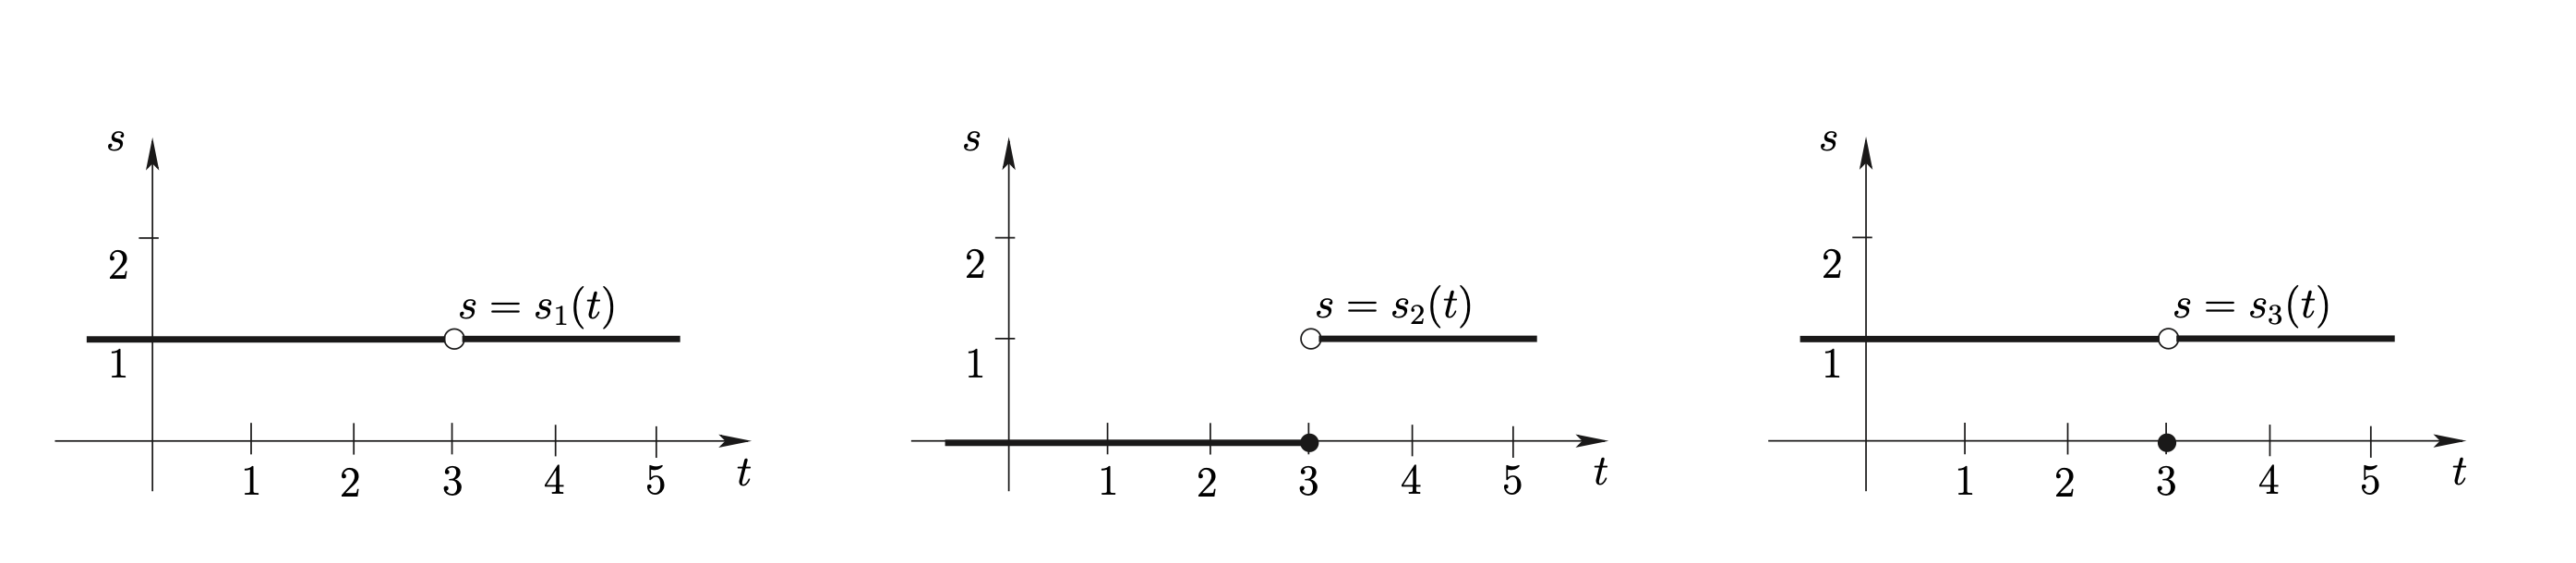
\includegraphics[width=0.5\linewidth]{images/fig-continuity-1} 

}

\caption{กราฟของฟังก์ชัน $s_1$, $s_2$ และ $s_3$}\label{fig:fig-continuity-1}
\end{figure}

\begin{definition}

ให้ \(f:D_{f}\rightarrow R\) โดยที่ \(D_{f}\subseteq R\) และ \(a\in R\) เรากล่าวว่า
\(f\) ต่อเนื่อง (cotinuous) ที่ \(a\) ถ้า

\begin{enumerate}
\def\labelenumi{\arabic{enumi}.}
\item
  \(f \left( a\right)\) หาค่าได้
\item
  \(\underset{x\rightarrow a}{\lim}f(x)\) หาค่าได้
\item
  \(f\left( a\right) =\underset{x\rightarrow a}{\lim}f(x)\)
\end{enumerate}

\end{definition}

\begin{definition}
ให้ \(f\) เป็น function และ \(S\) เป็นเซต (set) เรากล่าวว่า \(f\) ต่อเนื่องบน \(S\)
(continuous on \(S\)) ถ้า \(f\) ต่อเนื่องที่ทุก ๆ สมาชิกของ \(S\) เรียก function ที่
continuous on \(R\) ว่า ``ฟังก์ชันต่อเนื่อง (continuous function)''
\end{definition}

\textbf{ข้อสังเกต} จะเห็นว่า function ที่แสดงตำแหน่งของวัตถุต้องเป็น continuous function
บนช่วงที่สนใจ

\begin{theorem}
\protect\hypertarget{thm:thm-cont-1}{}\label{thm:thm-cont-1}

ถ้า \(f\) และ \(g\) เป็น function ที่ต่อเนื่องที่ \(a\) แล้ว

\begin{enumerate}
\def\labelenumi{\arabic{enumi}.}
\item
  \(f+g\) ต่อเนื่องที่ \(a\)
\item
  \(f-g\) ต่อเนื่องที่ \(a\)
\item
  \(f\cdot g\) ต่อเนื่องที่ \(a\)
\item
  \(\frac{f}{g}\) ต่อเนื่องที่ \(a\) ถ้า \(g\left( a\right) \neq 0\)
\end{enumerate}

\end{theorem}

\begin{example}
\protect\hypertarget{exm:ex-cont-1}{}\label{exm:ex-cont-1}function \(f\) ซึ่งนิยามโดย \(f\left( x\right) =\left| x\right|\)
เป็นฟังก์ชันต่อเนื่องหรือไม่
\end{example}

\textbf{วิธีทำ} ในที่นี้ \[f\left( x\right) =
             \begin{cases}
            x & \text{ ถ้า } x \ge 0 \\
            -x  & \text{ ถ้า } x>0
              \end{cases}\] เราต้องพิจารณาว่า \(f\) ต่อเนื่องที่ทุก ๆ \(a\in R\)
หรือไม่

\begin{itemize}
\item
  ถ้า \(a>0\) จะได้
  \(\underset{x\rightarrow a}{\lim}f(x)=\underset{x\rightarrow a}{\lim}x=a=f(a)\)
\item
  ถ้า \(a<0\) จะได้
  \(\underset{x\rightarrow a}{\lim}f(x)=\underset{x\rightarrow a}{\lim}(-x)=-a=f(a)\)
\item
  ถ้า \(a=0\)จะได้
  \(\underset{x\rightarrow 0^{-}}{\lim}f(x)=\underset{x\rightarrow 0^{-}}{\lim}(-x)=0=f(0)\)\\
  และ
  \(\underset{x\rightarrow 0^{+}}{\lim}f(x)=\underset{x\rightarrow 0^{+}}{\lim}x=0=f(0)\)\\
  ดังนั้น \(\underset{x\rightarrow 0}{\lim}f(x)=0=f(0)\)
\end{itemize}

ดังนั้น \(f\) ต่อเนื่องที่ทุก ๆ \(a\in R\) จึงสรุปว่า \(f\) เป็น continuous function

\begin{theorem}
\protect\hypertarget{thm:thm-cont-2}{}\label{thm:thm-cont-2}ฟังก์ชันตรรกยะ (rational function) เป็น function ที่ต่อเนื่องบน domain ของมัน
\end{theorem}

\textbf{หมายเหตุ}: rational function คือ function ที่เป็นเศษส่วนของพหุนาม
(polynomial) domain ของ rational function
ได้แก่เซตของจำนวนจริงซึ่งไม่ทำให้ส่วนของมันเป็นศูนย์

\begin{theorem}
\protect\hypertarget{thm:thm-cont-3}{}\label{thm:thm-cont-3}ถ้า \(f\) และ \(g\) เป็น function และ \(a\in R\) โดยที่
\(\underset{x\rightarrow a}{\lim}g(x)=L\) และ \(f\) ต่อเนื่องที่ \(L\) แล้ว
\(\underset{x\rightarrow a}{\lim}f(g(x))=f(\underset{x\rightarrow a}{\lim}g(x))=f(L)\)
\end{theorem}

\begin{example}
\protect\hypertarget{exm:ex-cont-2}{}\label{exm:ex-cont-2}\(\underset{x\rightarrow 1}{\lim}\left| \frac{x^{4}-x^{2}+1}{x^{4}+x^{2}+1}\right| =?\)
\end{example}

\textbf{วิธีทำ} 

\begin{equation}
  \begin{aligned}
    \underset{x\rightarrow 1}{\lim}\left| \frac{x^{4}-x^{2}+1}{x^{4}+x^{2}+1}\right|
    &=\left| \ \underset{x\rightarrow 1}{\lim}\frac{x^{4}-x^{2}+1}{x^{4}+x^{2}+1}\right| \\
    &=\left| \frac{1^{4}-1^{2}+1}{1^{4}+1^{2}+1}\right| \\
    &=\left| \frac{1}{3}\right| =\frac{1}{3}
  \end{aligned}
\end{equation}

\begin{theorem}
\protect\hypertarget{thm:thm-cont-4}{}\label{thm:thm-cont-4}ถ้า \(f\) ต่อเนื่องที่ \(a\) และ \(g\) ต่อเนื่องที่ \(f(a)\) แล้ว \(g\circ f\) ต่อเนื่องที่ \(a\)
\end{theorem}

\textbf{จงพิสูจน์ทฤษฎีบทข้างต้น}

\begin{example}
\protect\hypertarget{exm:ex-cont-3}{}\label{exm:ex-cont-3}function f ซึ่งนิยามโดย
\(\ f\left( x\right) =\left| \frac{x^{4}-x^{2}+1}{x^{4}+x^{2}+1}\right|\)
เป็น continuous function หรือไม่
\end{example}

\textbf{วิธีทำ} \(f\) เป็น continuous function เพราะ \(f =g\circ h\) โดยที่
\(g\left( x\right) =\left| x\right|\) และ
\(h\left( x\right) =\frac{x^{4}-x^{2}+1}{x^{4}+x^{2}+1}\) ซึ่งเป็น continuous
function ทั้งคู่

\begin{definition}

เรานิยาม ``ภาวะต่อเนื่องทางซ้าย'' และ ``ภาวะต่อเนื่องทางขวา'' ได้โดยแทนที่
\(\underset{x\rightarrow a}{\lim}\) ในเงื่อนไขของนิยาม ด้วย
\(\underset{x\rightarrow a^{-}}{\lim}\) และ
\(\underset{x\rightarrow a^{+}}{\lim}\) ตามลำดับ นั่นคือ

ให้ \(f:D_{f}\rightarrow R\) โดยที่ \(D_{f}\subseteq R\) และ \(a\in R\) เรากล่าวว่า
\(f\) ``ต่อเนื่องทางซ้าย (left-continuous) ที่ \(a\)'' ถ้า

\begin{enumerate}
\def\labelenumi{\arabic{enumi}.}
\item
  \(f\left( a\right)\) หาค่าได้
\item
  \(\underset{x\rightarrow a^{-}}{\lim}f(x)\) หาค่าได้
\item
  \(f\left( a\right) =\underset{x\rightarrow a^{-}}{\lim}f(x)\)
\end{enumerate}

และกล่าวว่า \(f\) ``ต่อเนื่องทางขวา (right-continuous) ที่ \(a\)'' ถ้า

\begin{enumerate}
\def\labelenumi{\arabic{enumi}.}
\item
  f\(\left( a\right)\) หาค่าได้
\item
  \(\underset{x\rightarrow a^{+}}{\lim}f(x)\) หาค่าได้
\item
  f\(\left( a\right) =\underset{x\rightarrow a^{+}}{\lim}f(x)\)
\end{enumerate}

\end{definition}

\begin{definition}

ให้ \(f : \left[ a,b\right] \rightarrow R\) เรากล่าวว่า \(f\) ต่อเนื่องบน
\(\left[ a,b\right]\) (continuous on \(\left[ a,b\right]\)) ถ้า

\begin{enumerate}
\def\labelenumi{\arabic{enumi}.}
\item
  \(f\) ต่อเนื่องบน \((a,b)\)
\item
  \(f\) ต่อเนื่องทางขวาที่ \(a\)
\item
  \(f\) ต่อเนื่องทางซ้ายที่ \(b\)
\end{enumerate}

\end{definition}

\begin{example}
\protect\hypertarget{exm:ex-cont-4}{}\label{exm:ex-cont-4}function \(f\) ที่นิยามโดย \(f\left( x\right) =\sqrt{4-x^{2}}\) เป็น continuous
function บน \(\left[ -2,2\right]\) หรือไม่
\end{example}

\textbf{วิธีทำ} เราตรวจสอบได้ว่า \(f\) เป็น continuous function บน
\(\left[ -2,2\right]\) เพราะ\\
1. \(f\) เป็น continuous function บน \(\left( -2,2\right)\)\\
2. \(f\) ต่อเนื่องทางขวาที่ -2 เพราะ \$\$

\begin{equation}
  \begin{aligned}
    \underset{x\rightarrow -2^{+}}{\lim}f(x)
        &=\underset{x\rightarrow -2^{+}}{\lim}\sqrt{4-x^{2}} \\
        &=0=f\left( -2\right)
  \end{aligned}
\end{equation}

\begin{enumerate}
\def\labelenumi{\arabic{enumi}.}
\setcounter{enumi}{2}
\tightlist
\item
  \(f\) ต่อเนื่องทางซ้าย ที่ 2 เพราะ
\end{enumerate}

\begin{equation}
  \begin{aligned}
        \underset{x\rightarrow -2^{-}}{\lim}f(x)
        &=\underset{x\rightarrow -2^{-}}{\lim}\sqrt{4-x^{2}} \\
        &=0 =f\left( 2\right)
  \end{aligned}
\end{equation}

\begin{example}
\protect\hypertarget{exm:ex-cont-5}{}\label{exm:ex-cont-5}

พิจารณา function f ซึ่งมีกราฟดังต่อไปนี้

\begin{figure}

{\centering 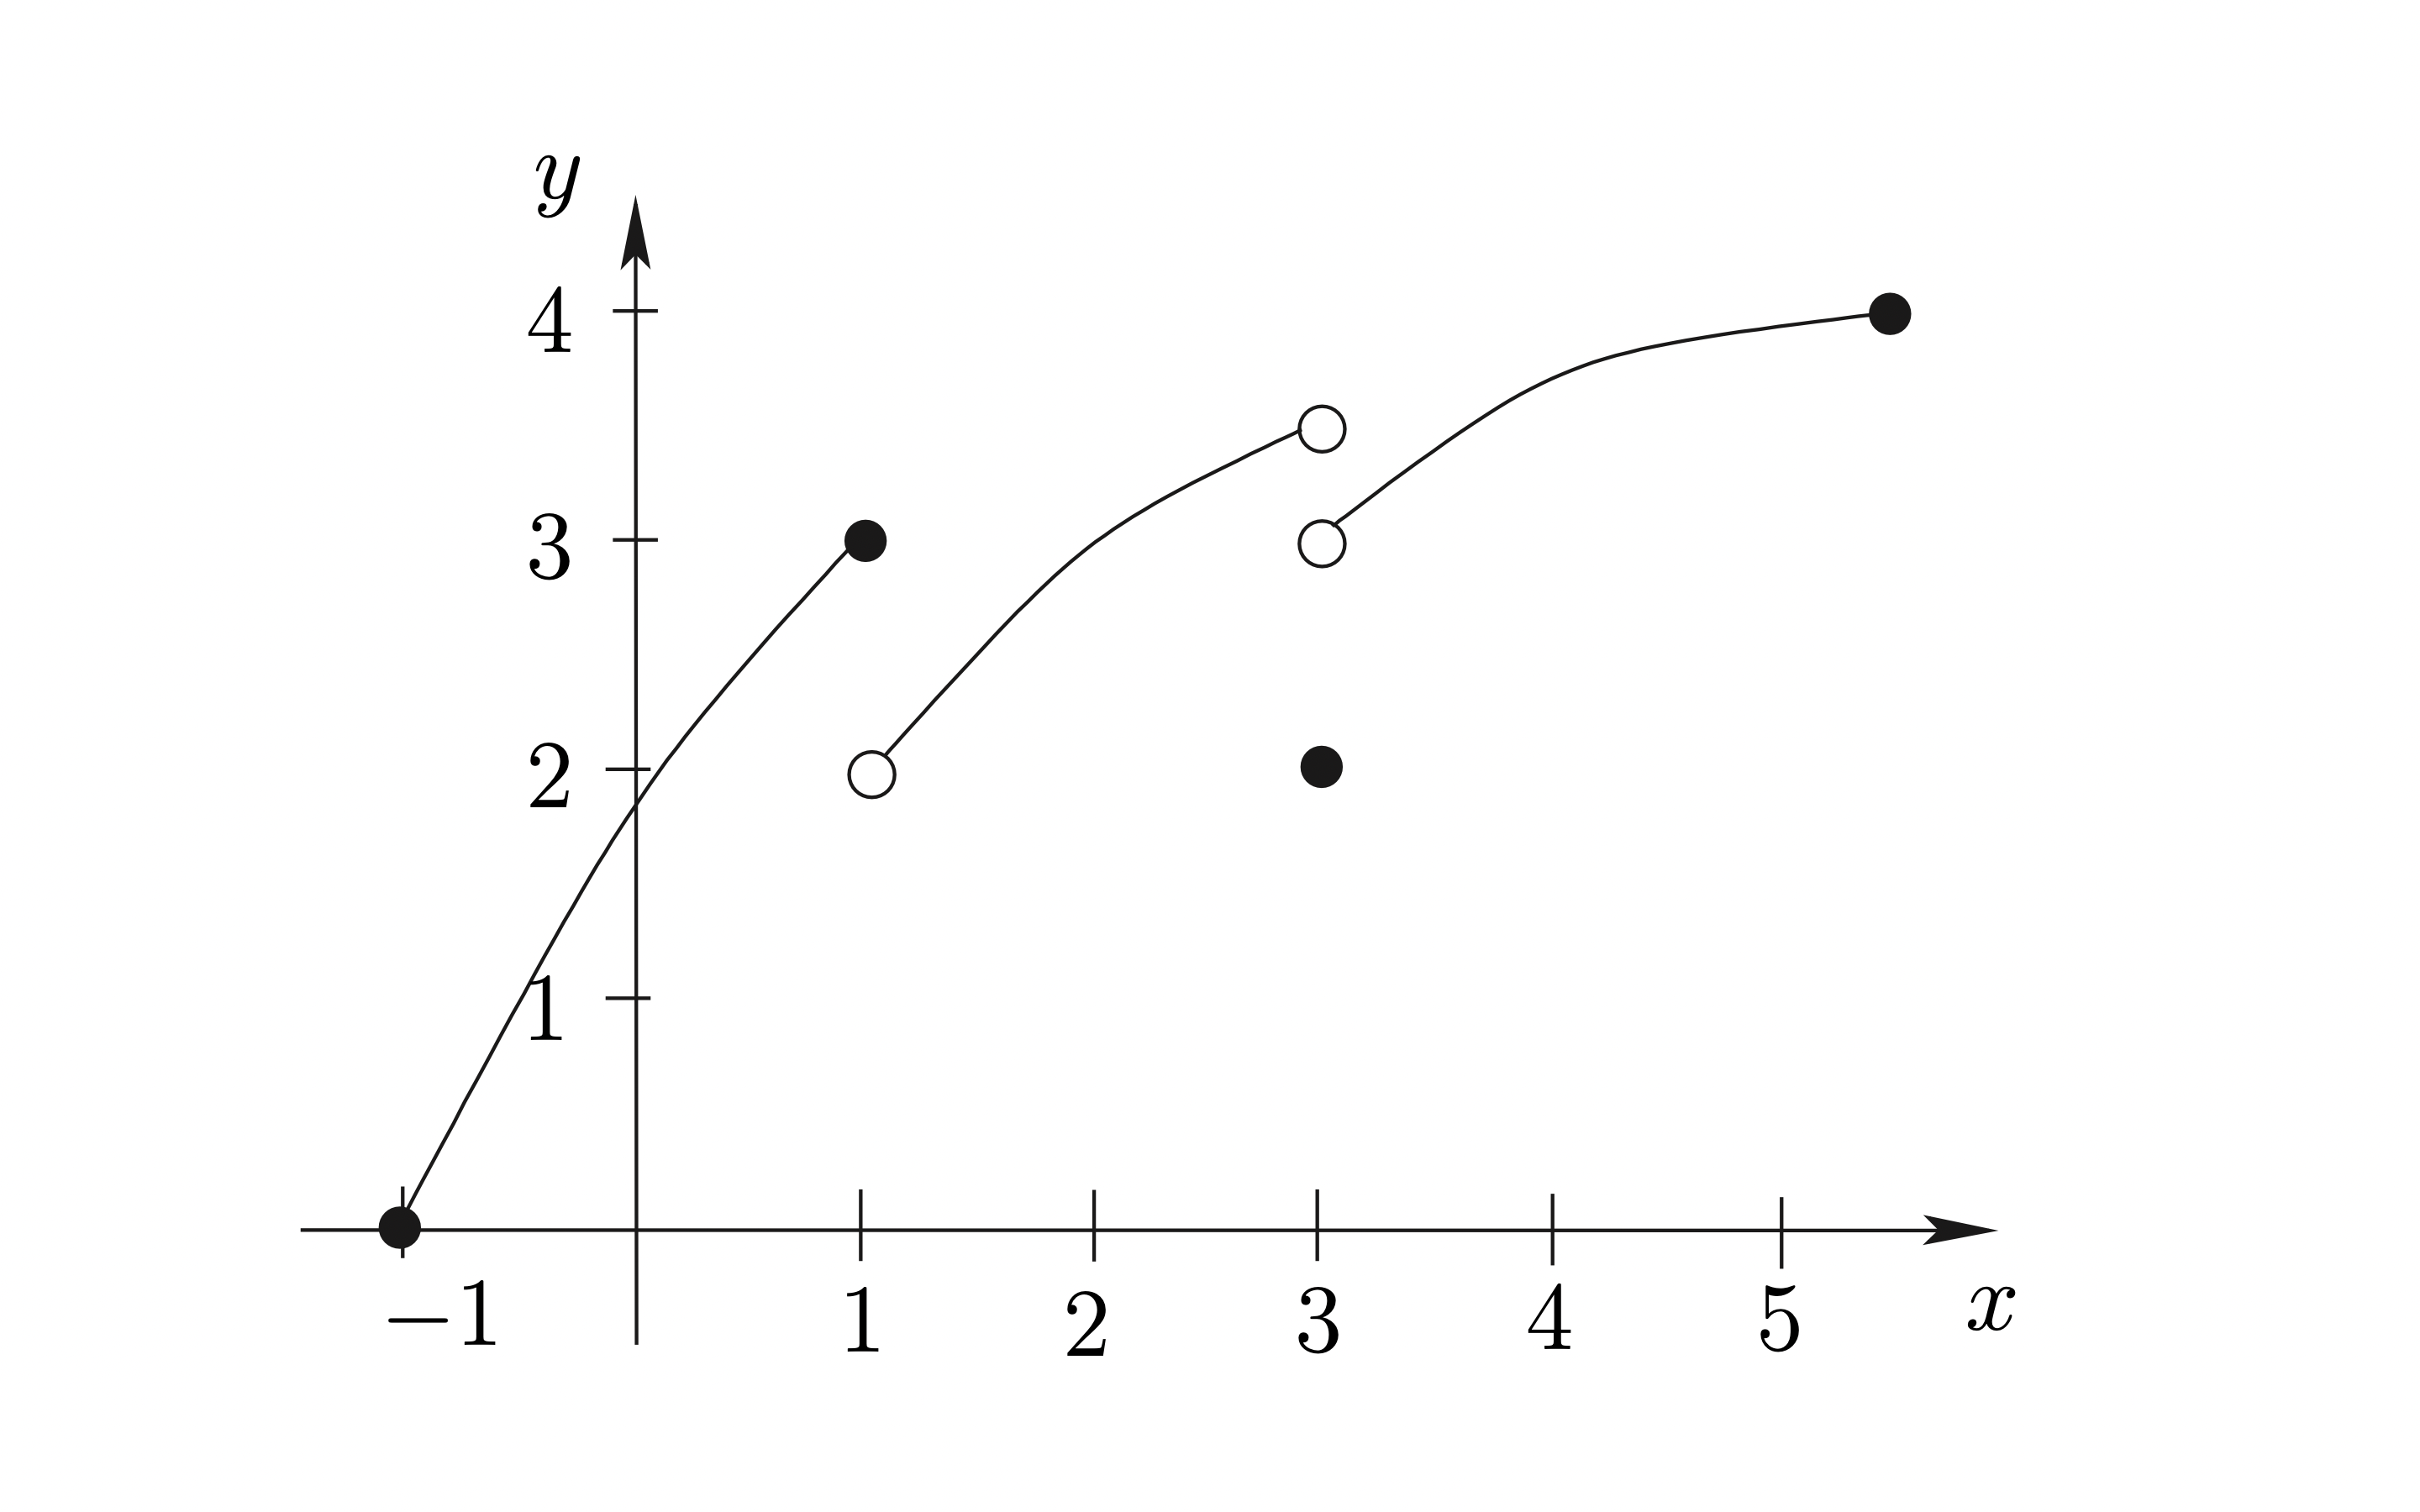
\includegraphics[width=0.5\linewidth]{images/fig-continuity-2} 

}

\caption{กราฟของฟังก์ชันในตัวอย่าง \\ref{exm:ex-cont-5}}\label{fig:fig-continuity-2}
\end{figure}

\begin{enumerate}
\def\labelenumi{\arabic{enumi}.}
\tightlist
\item
  \(f\) มีความต่อเนื่องที่ \(-1,0,1,2,3,4,5\) หรือไม่\\
\item
  \(f\) มีความต่อเนื่องบน
  \(\left[ -1,0\right] ,\left[ 0,1\right] ,\left[ 1,2\right] ,\left[ 2,3\right] ,\left[ 3,4\right] ,\left[ 4,5\right]\)
  หรือไม่
\end{enumerate}

\end{example}

\textbf{วิธีทำ} ให้นักศึกษาทำเป็นแบบฝึกหัด

\begin{theorem}
\protect\hypertarget{thm:thm-cont-5}{}\label{thm:thm-cont-5}ฟังก์ชันตรีโกณมิติ ฟังก์ชันตรีโกณมิติผกผัน ฟังก์ชันเลขชี้กำลัง และฟังก์ชันลอการิทึม
เป็นฟังก์ชันที่ต่อเนื่องบนโดเมนของมัน
\end{theorem}

  \bibliography{book.bib}

\end{document}
